\section{Dimensionamento preliminare}
\begin{figure}[H]
\centering
  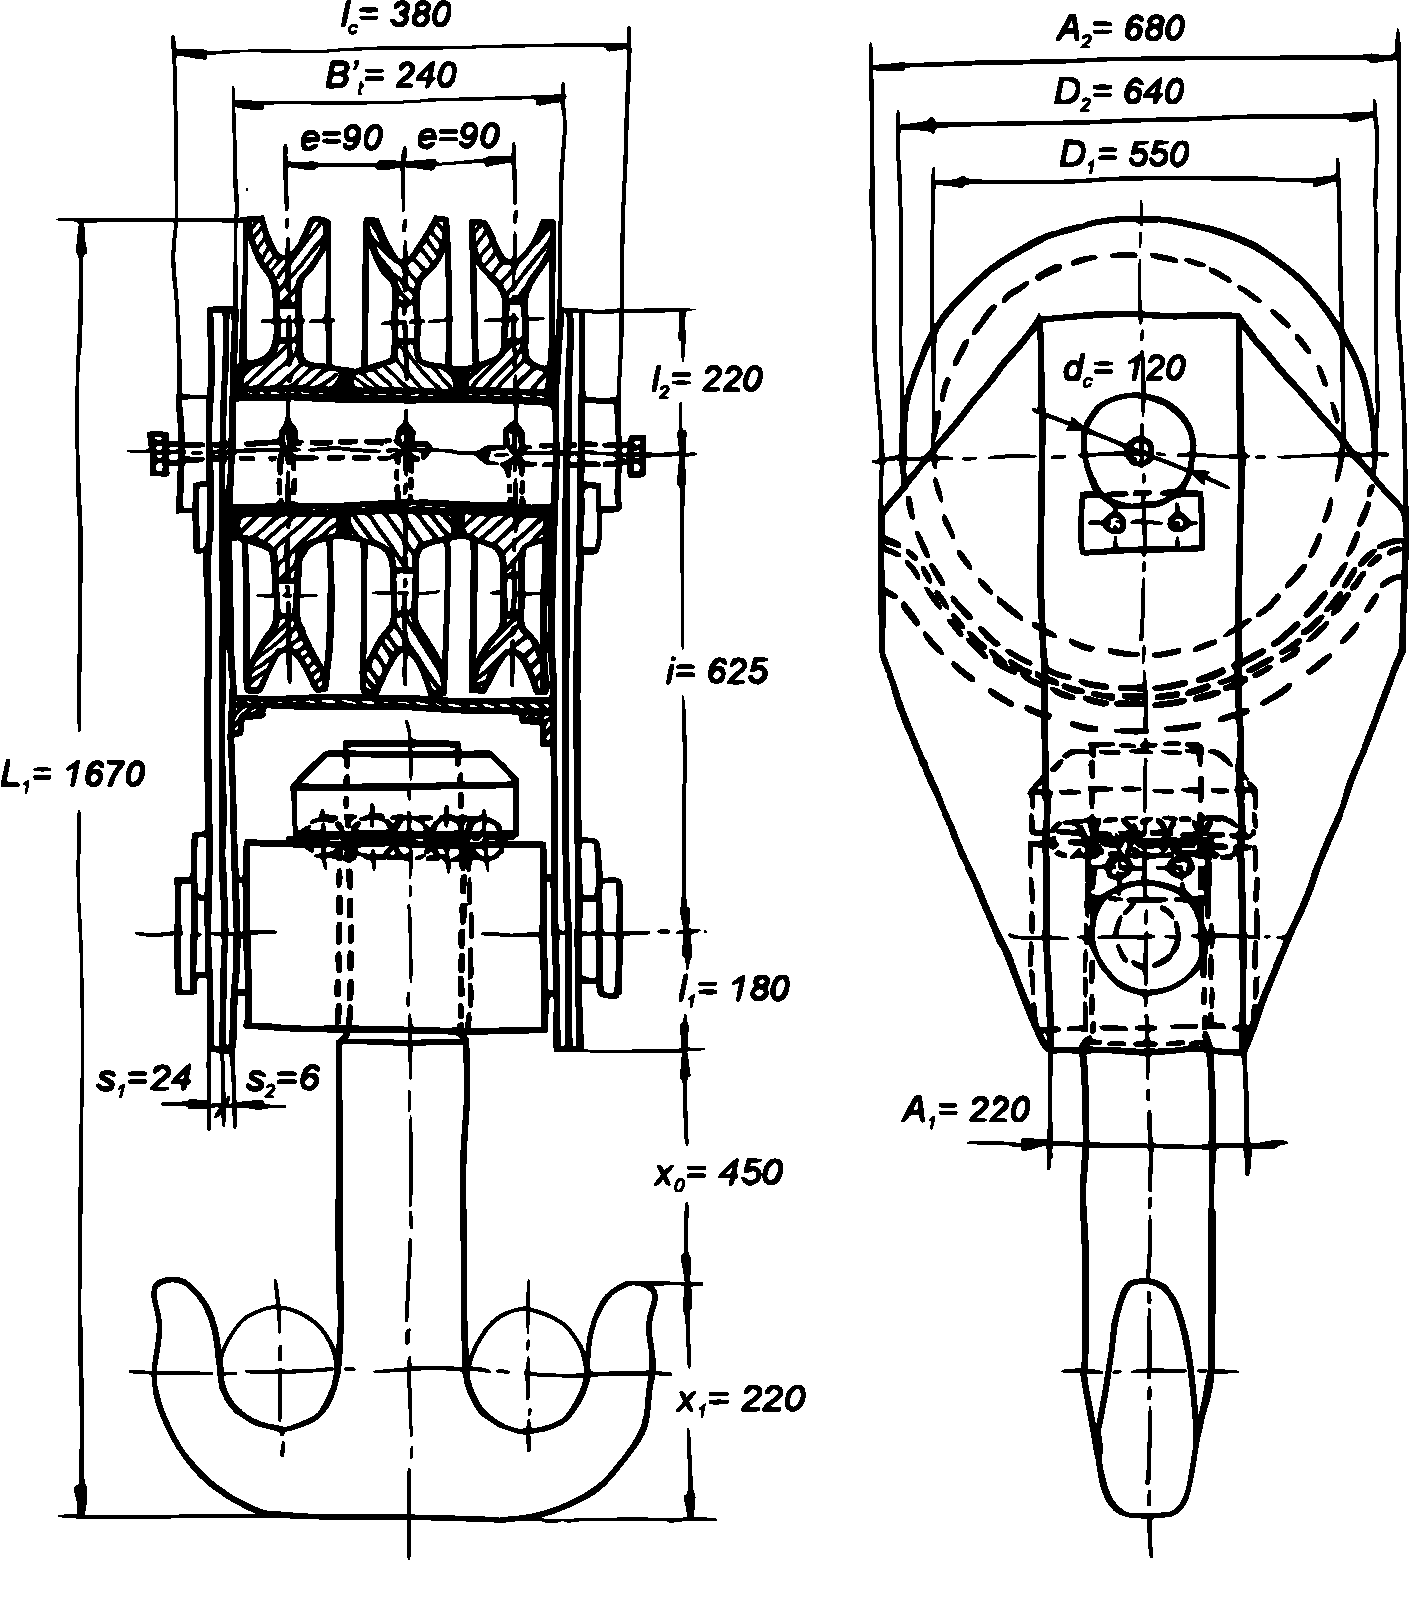
\includegraphics[width=.5\textwidth]{imgs/Cap5/1 DimPrel}
\caption{Dimensioni principali del bozzello.}
\label{fig:DimPrel1}
\end{figure}
\begin{figure}[H]
\centering
  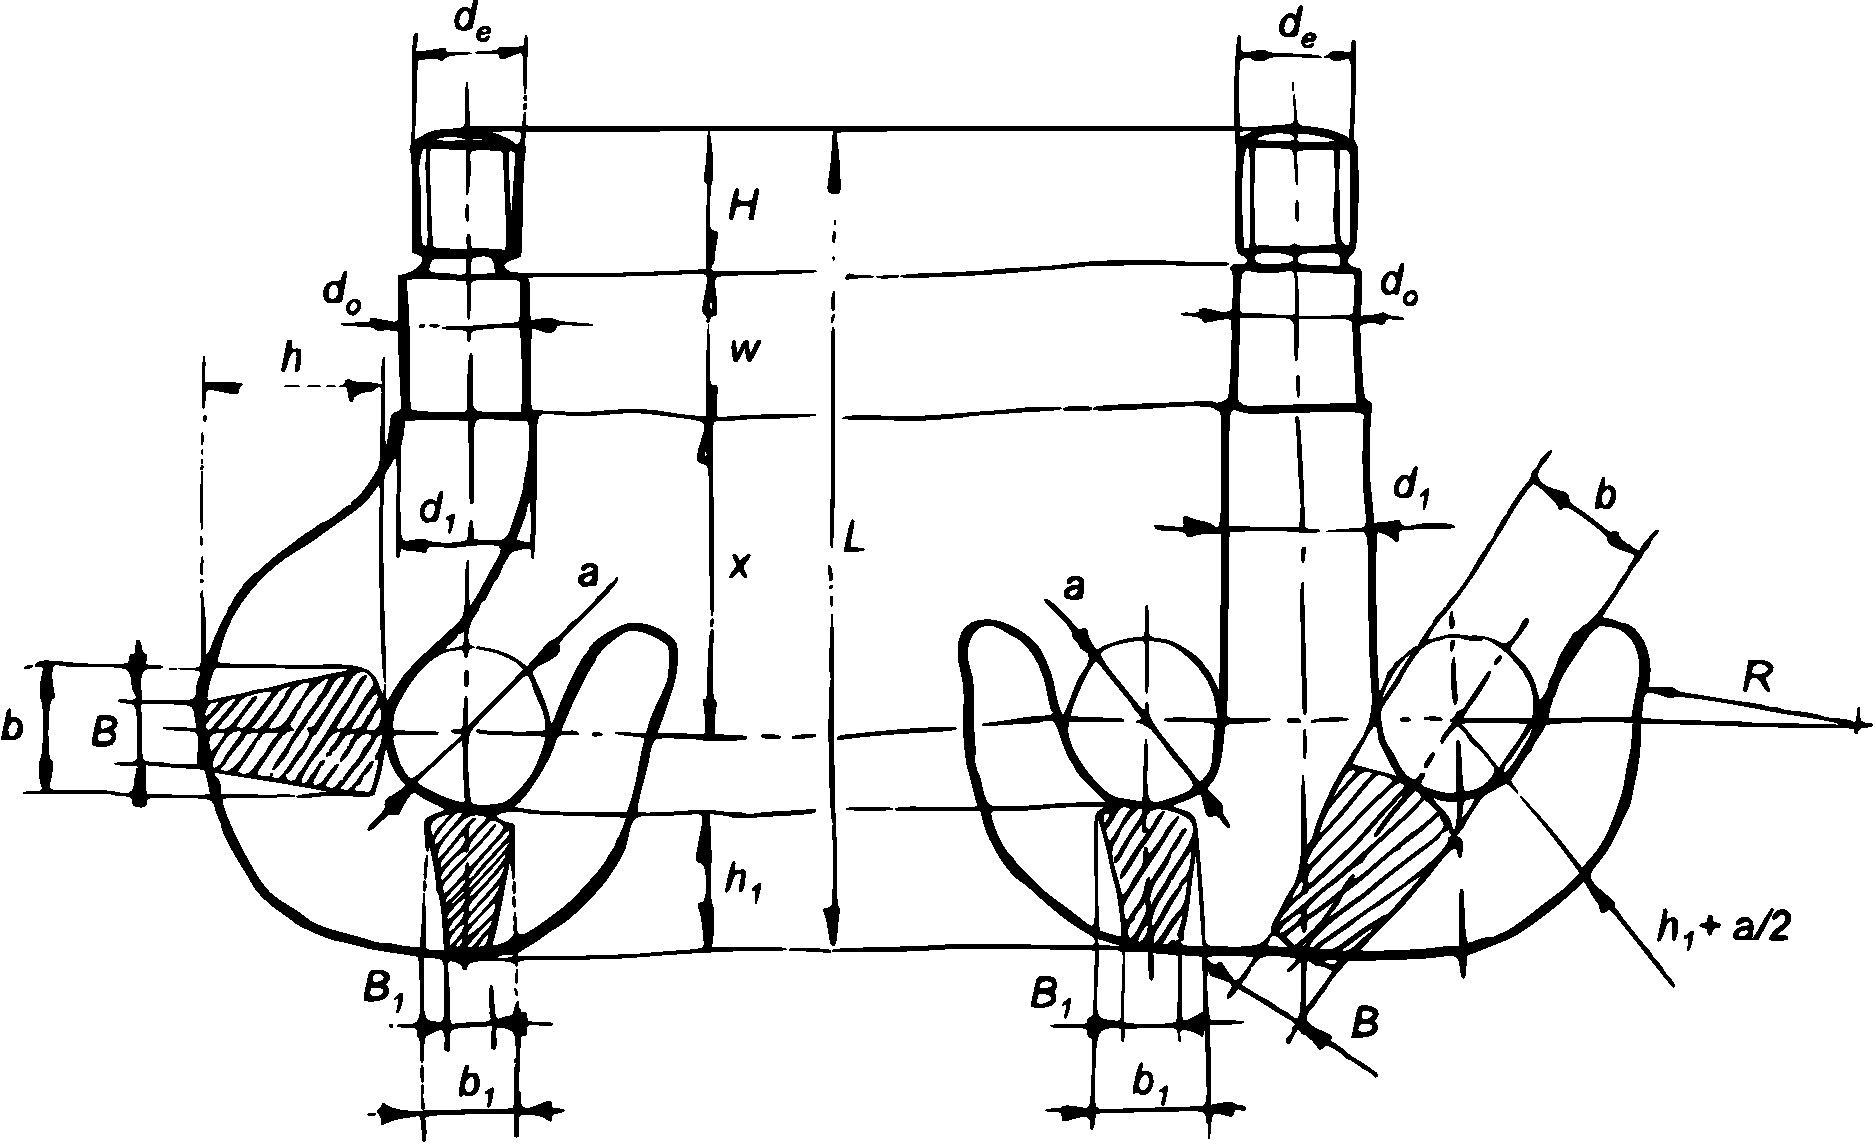
\includegraphics[width=.6\textwidth]{imgs/GancioGen}
\caption{Dimensioni principali del gancio.}
\label{fig:GancioGen}
\end{figure}
In prima battuta risulta molto utile studiare le tipologie di bozzello con gancio presenti sul mercato.
Nei prossimi paragrafi si utilizzeranno diverse tabelle per effetturare un dimensionamento preliminare; tali tabelle sono basate sull'esperienza dei costrutturi. 
In questo modo si possiede una linea guida per determinare le dimensioni di massima del progetto. 

I ganci disponibili in commercio sono realizzati in acciaio fucinato, possono essere a becco singolo o a becco doppio. 
Dalla normativa sulla sicurezza per i dispositivi di sollevamento è previsto un sistema di ritenuta del carico. 
Il numero di carrucole impiegate è in relazione con i tiri di fune e quindi con la portata utile. Tali carrucole vengono prodotte in ghisa sferoidale per fusione.
La gola viene realizzata con macchina utensile, sono poi presenti dei fori di alleggerimento equidistanziati angolarmente rispetto all'asse di rotazione. 
Le carrucole sono folli sull'asse di calettamento, quest'ultimo avviene attraverso boccole flangiate in bronzo adeguatamente lubrificate. Il lubrificante viene apportato attraverso dei fori di adduzione praticati sull'asse.

L'inscatolamento del sistema avviene attraverso coppie di lamoni e piastroni. Nella parte superiore vengono ospitate le carrucole, mentre nella parte inferiore è presente la traversa forata per permettere il passaggio del gambo filettato del gancio. Viene previsto quindi un dado che andrà ad appoggiarsi sulla traversa attraverso un cuscinetto a sfere reggispinta. Il carico viene quindi trasmesso dal gancio alla traversa attraverso il dado, dalla traversa ai lamoni piastroni e quindi all'asse. L'asse trasmette il carico alle carrucole e quindi alle funi che trasmettono una forza uguale e contraria equilibrando il sistema.

Il cuscinetto a sfere presente tra dado e traversa ha una doppia funzione: evitare dannose torsioni dei tiri di fune e permettere all'operature di ruotare il gancio per agganciare il carico.
Al fine di garantire la libera rotazione delle carrucole deve essere previsto un gioco tra le boccole. 
Al di sotto delle carrucole e al di sopra della traversa sono previsti dei carter di irrigidimento, si adotteranno poi anche degli irrigidimenti laterali avendo cura di lasciare una luce per lo scolo dell'acqua piovana tra irrigidimenti laterali e carter inferiore. Sono presenti poi dei distanziali cilindrici forati, al cui interno verranno posti dei cilindri filettati che andranno ad avvitarsi sui piastroni con dado e rosetta fungendo da tiranti, questi hanno la funzione di irrigidire ulteriormente il sistema. 

Per impedire l'eventuale traslazione assiale dell'asse viene prevista una tasca sullo stesso all'interno della quale ha sede una piastrina che viene avvitata al lamone. 
Deve essere impedito lo spostamento assiale anche alla traversa ma senza impedirne la rotazione sul proprio asse, il bloccaggio avviene sempre con piastrina. 

Il calettamento delle boccole sulle carrucole è con interferenza mentre l'accoppiamento boccola-asse è con gioco. Tra il gambo del gancio e il foro della traversa è presente gioco. Il cambo del gancio presenta uno spallamento funzionale che entra in contatto con la traversa non appena il gancio si solleva verso la traversa. Questo è utile al fine di evitare il contatto tra gambo del gancio e carter inferiore.

Infine, per meglio definire i criteri di progettazione è possibile fare riferimento ai modelli presenti sul mercato. 
\begin{figure}[H]
\centering
  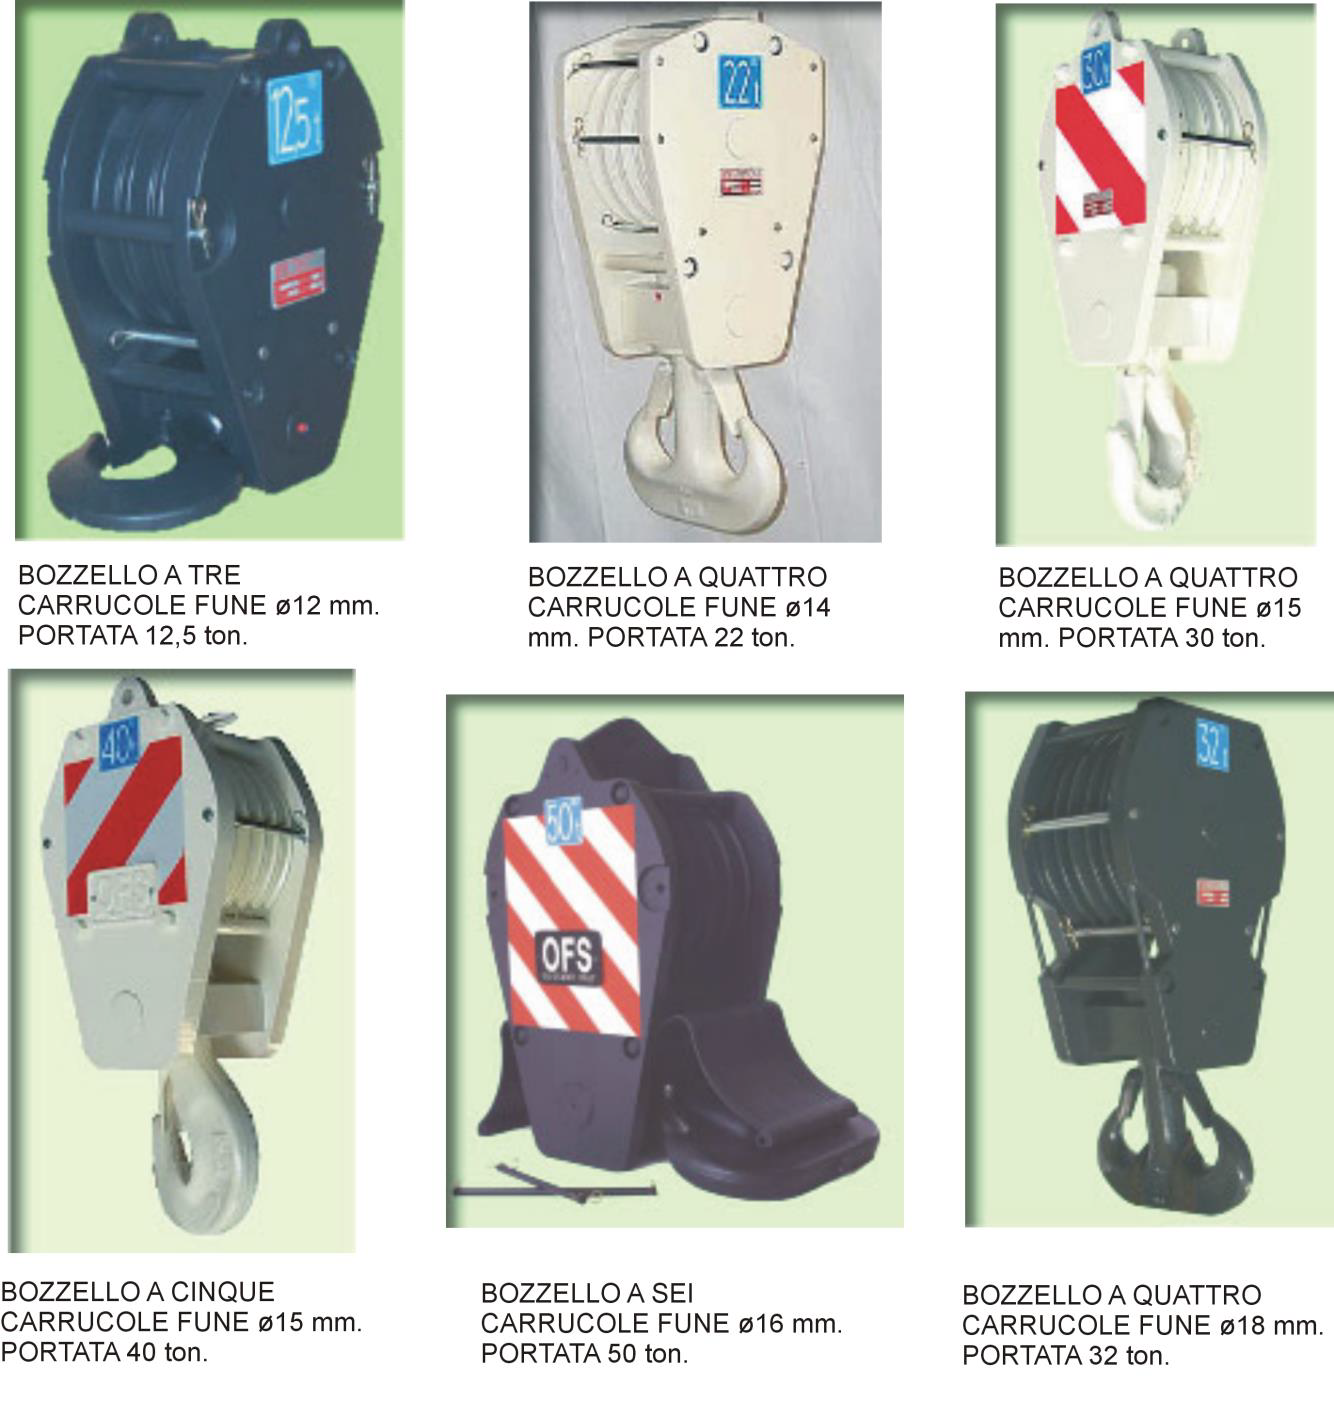
\includegraphics[width=.55\textwidth]{imgs/Esempi1}
\caption{}
\label{fig:Esempi1}
\end{figure}
\begin{figure}[H]
\centering
  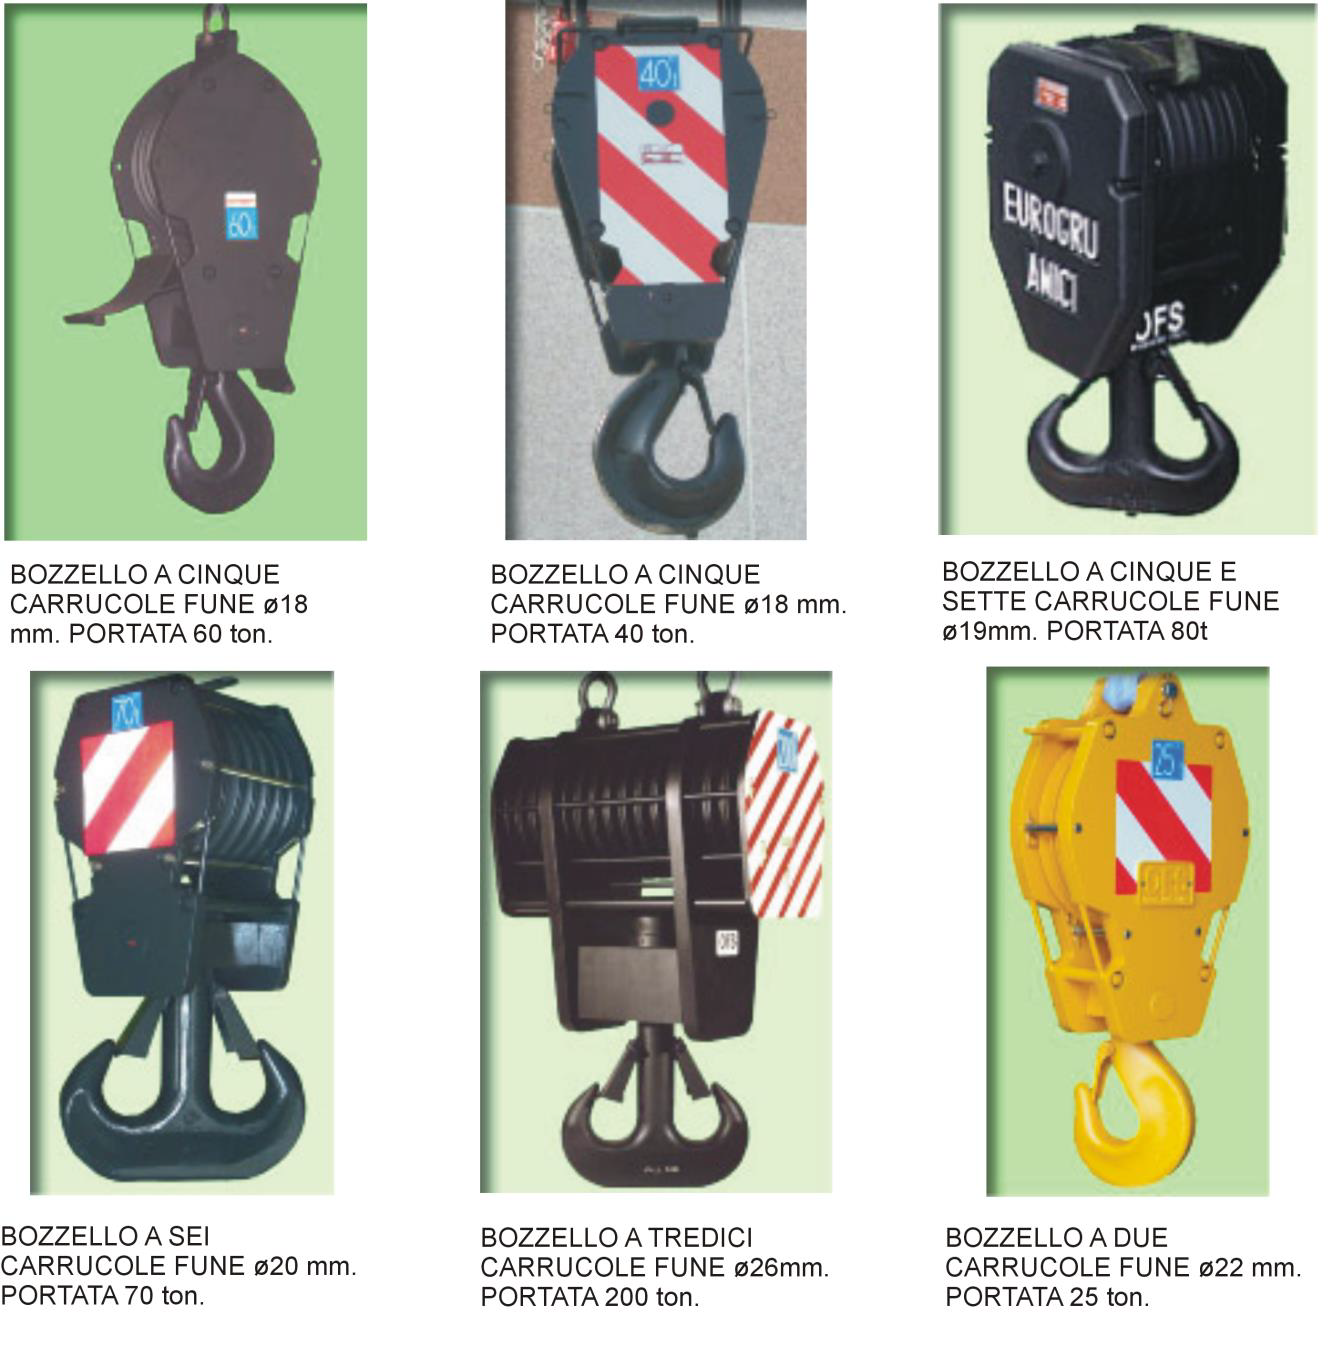
\includegraphics[width=.55\textwidth]{imgs/Esempi2}
\caption{}
\label{fig:Esempi2}
\end{figure}
\subsection{Dimensionamento generale}
Di seguito sono riportati i dati di progeto:
\begin{itemize}
\item Portata: 55 tonnellate;
\item Velocità di sollevamento: $5 \; m/min$.
\end{itemize}

In base alla documentazione rispetto ai modelli presenti sul mercato si procede con la progettazione di un gancio a due becchi.
Si passa ora alla scelta delle funi, il DPR 459 1996 sulla sicurezza dei dispositivi di sollevamento prevede un fattore di sicurezza pari a 5. 
In figura \ref{fig:TabellaFuni} è riportata la tabella con la capacità delle funi da catalogo Teci \footnote{http://www.teci.it/funi/speciali-a-trefoli/s12/}. 
\begin{figure}[H]
\centering
  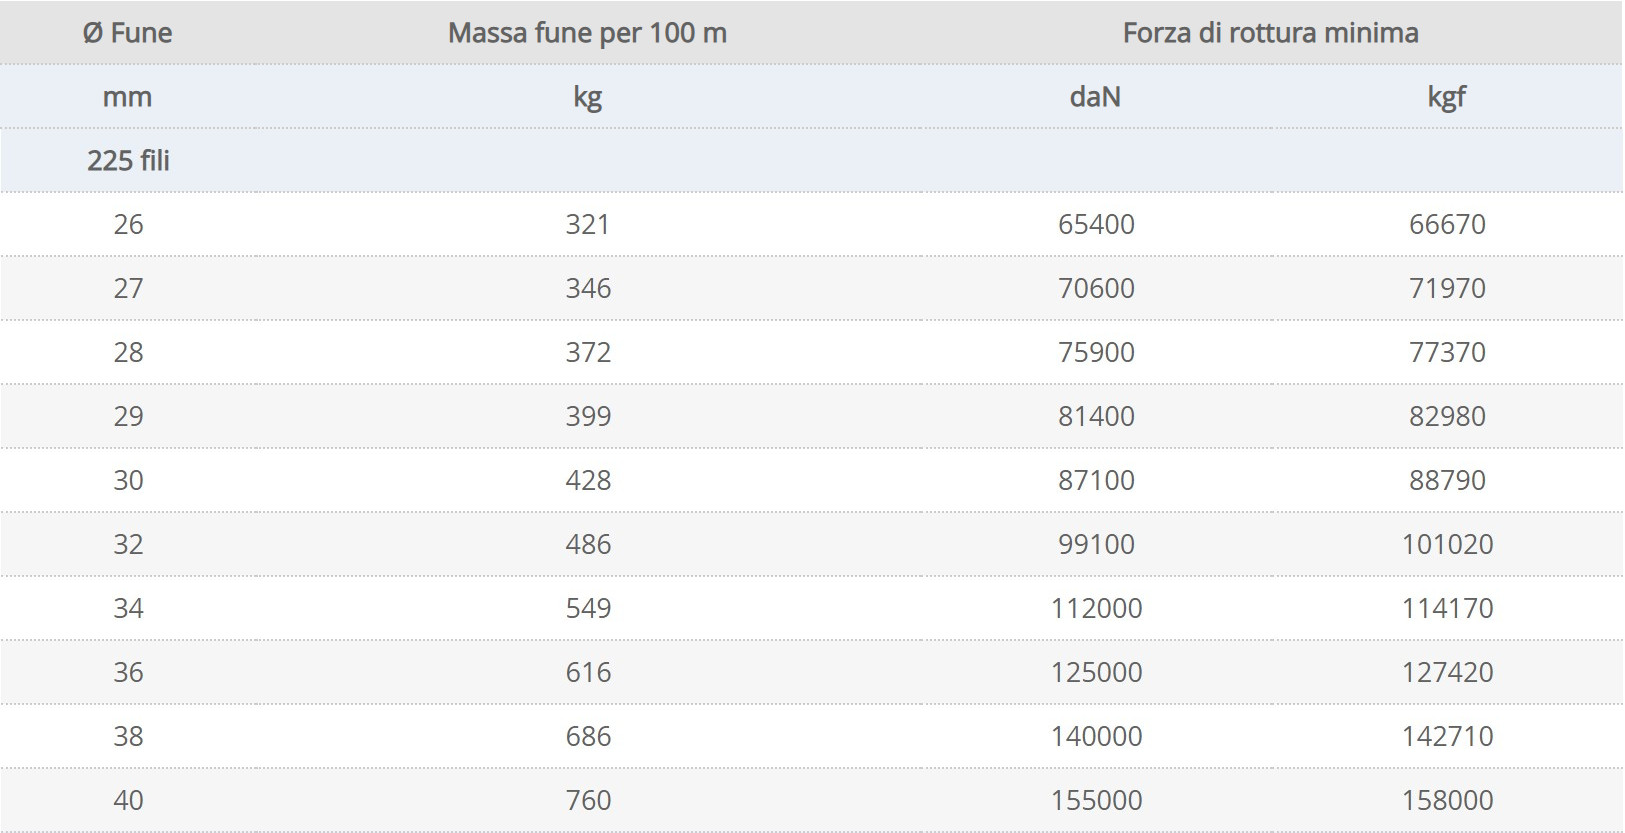
\includegraphics[width=.65\textwidth]{imgs/TabellaFuni}
\caption{Catalogo funi Teci, modello S12, 225 fili.}
\label{fig:TabellaFuni}
\end{figure}
\begin{figure}[H]
\centering
  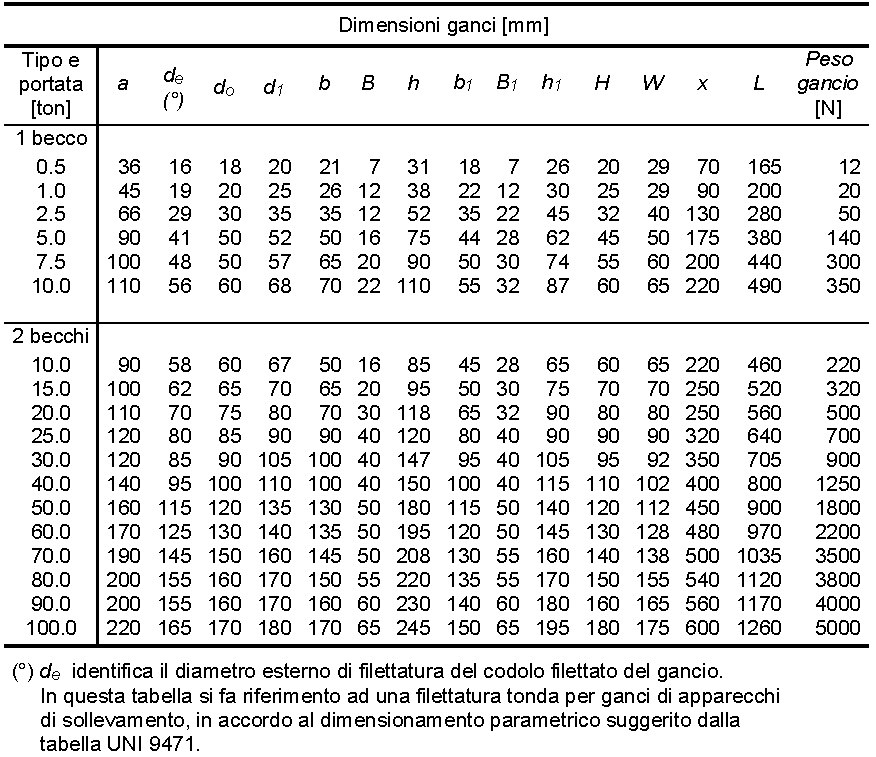
\includegraphics[width=.65\textwidth]{imgs/DimGen0}
\caption{Dimensioni generali riferite alla figura \ref{fig:GancioGen}.}
\label{fig:TabellaFuni}
\end{figure}
\begin{figure}[H]
\centering
\begin{minipage}{.5\textwidth}
  \centering
  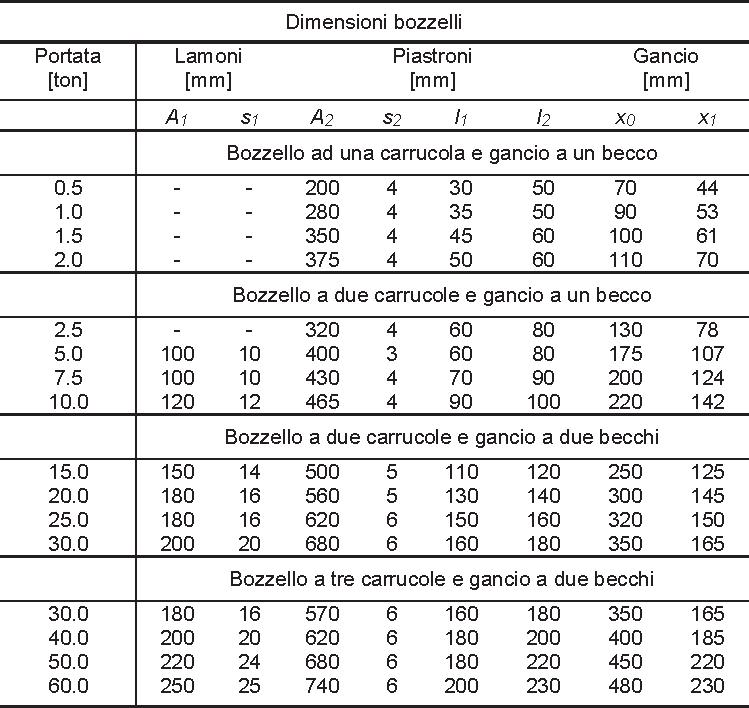
\includegraphics[width=.7\linewidth]{imgs/DimGen.pdf}
  \captionof{figure}{Dimensioni generali dei bozzelli con gancio.}
  \label{fig:DimGen0}
\end{minipage}%
\begin{minipage}{.5\textwidth}
  \centering
  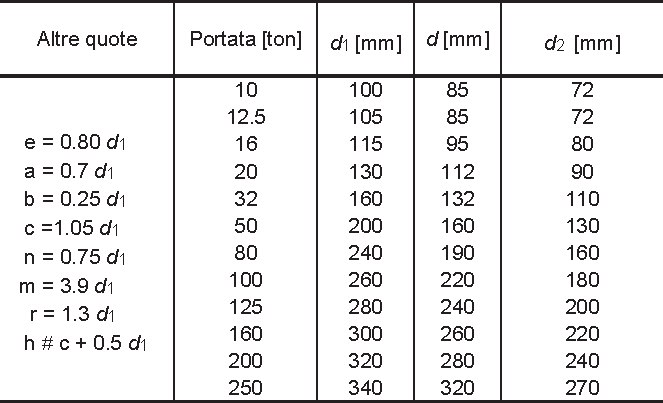
\includegraphics[width=.9\linewidth]{imgs/DimGen2.pdf}
  \captionof{figure}{Dimensioni generali dei ganci doppi.}
  \label{fig:DimGen2}
\end{minipage}
\end{figure}
Si è scelto di utilizzare tre carrucole con funi di acciaio di $26 \; mm$ di diametro. Da catalogo, la fune ha infatti una forza di rottura minima pari a $66670 \; kgf$. Il carico nominale è pari a $55000\;kgf$, utilizzando 3 cattucole si hanno 6 tiri di fune. Si divide allora il carico nominale per il numero di tiri di fune e si moltiplica per il fattore di sicurezza, si ottiene un valore di sollecitazione di $55000 \cdot 5/6 = 45833\; [kgf]$, un valore accettabile. 

Si passa ora al dimensionamento preliminare del gancio con i dati presenti in letteratura. 
Dalle tabelle in figura \ref{fig:DimGen} e \ref{fig:DimGen2}, tramite interpolazione si pssono ricavare le quote di massima di gancio e bozzello. Inserendolo il diametro del gambo del gancio nella tabella in figura \ref{fig:DimGambo} è possibile ricavarsi le quote generali del gambo stesso. 
\begin{figure}[H]
\centering
\begin{minipage}{.4\textwidth}
  \centering
  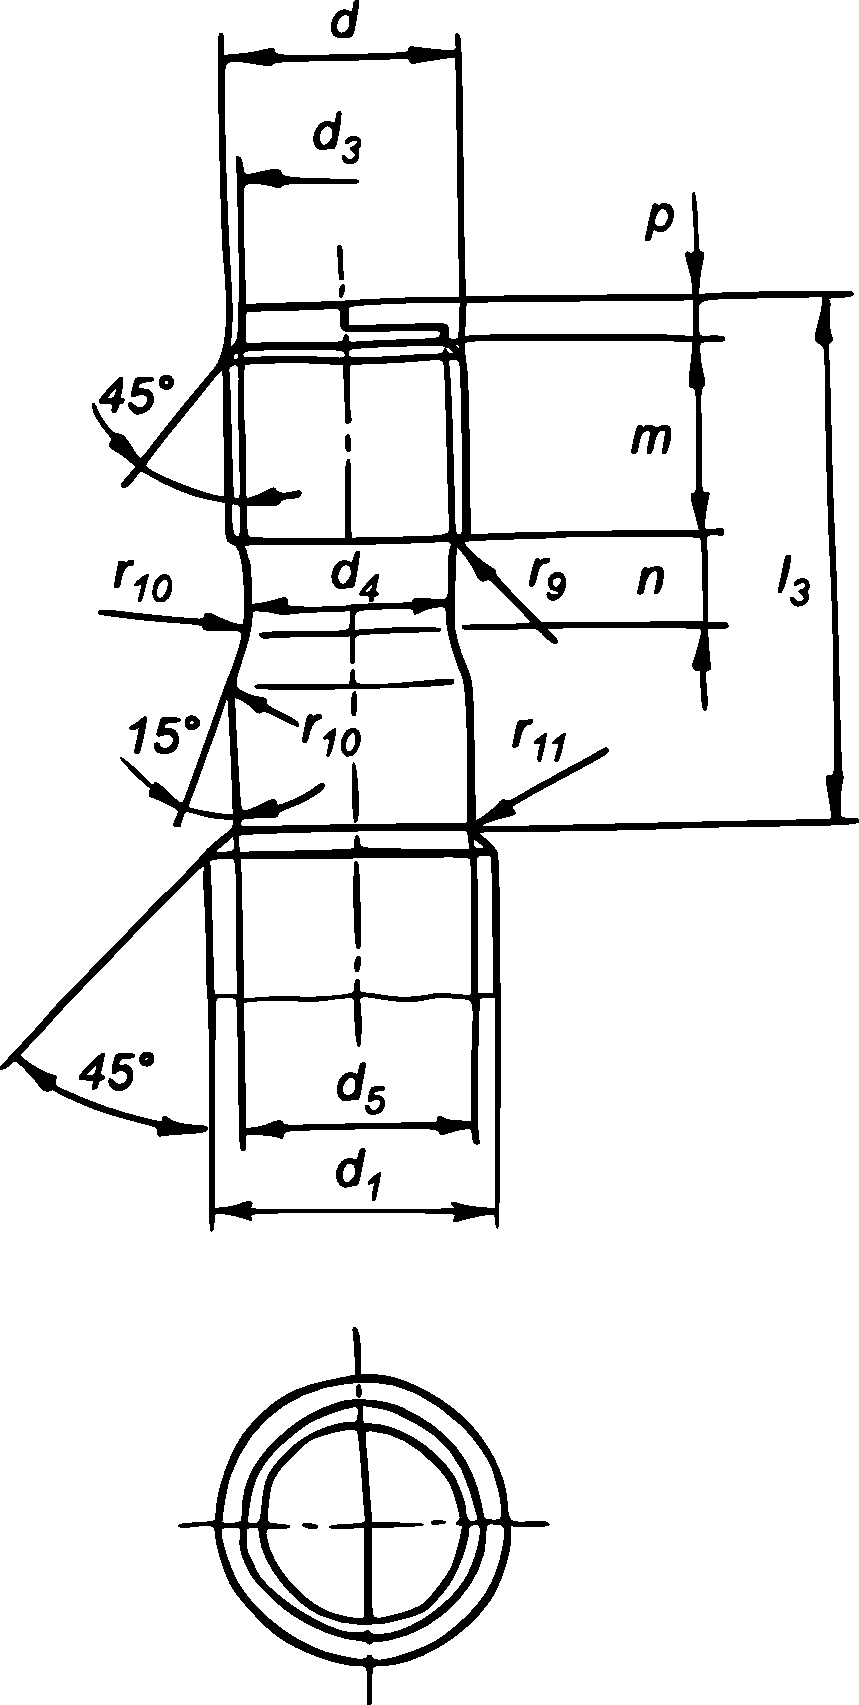
\includegraphics[width=.7\linewidth]{imgs/GamboDraw}
  \captionof{figure}{Gambo del gancio.}
  \label{fig:GamboDraw}
\end{minipage}%
\begin{minipage}{.6\textwidth}
  \centering
  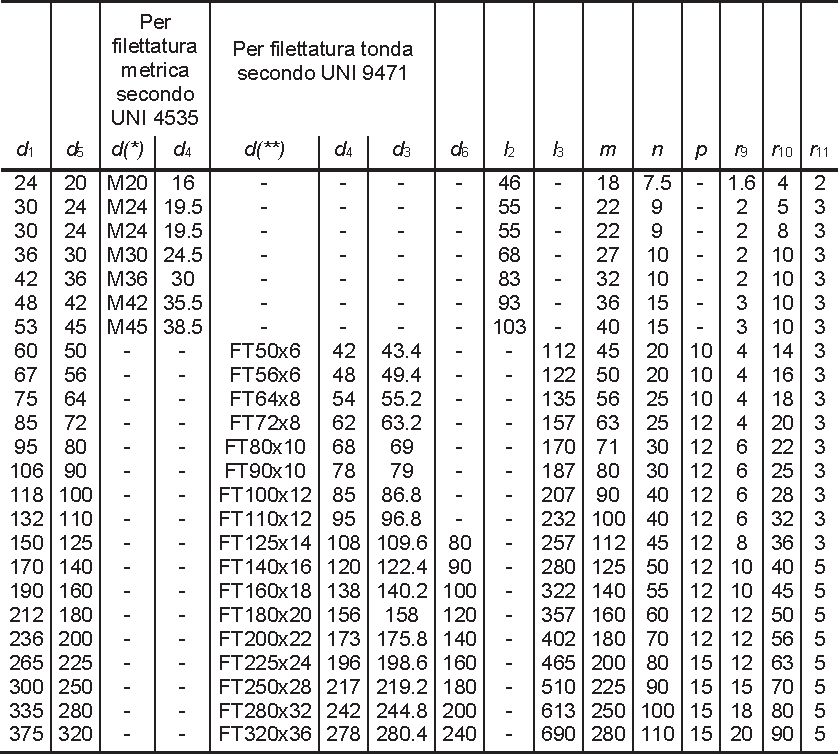
\includegraphics[width=.9\linewidth]{imgs/DimGambo}
  \captionof{figure}{Valori delle quote del gambo del gancio. Si noti che in questa tabella $d_1$ equivale a $d$ nella tabella \ref{fig:DimGen2}.}
  \label{fig:DimGambo}
\end{minipage}
\end{figure}

\begin{figure}[H]
\centering
\begin{minipage}{.45\textwidth}
  \centering
  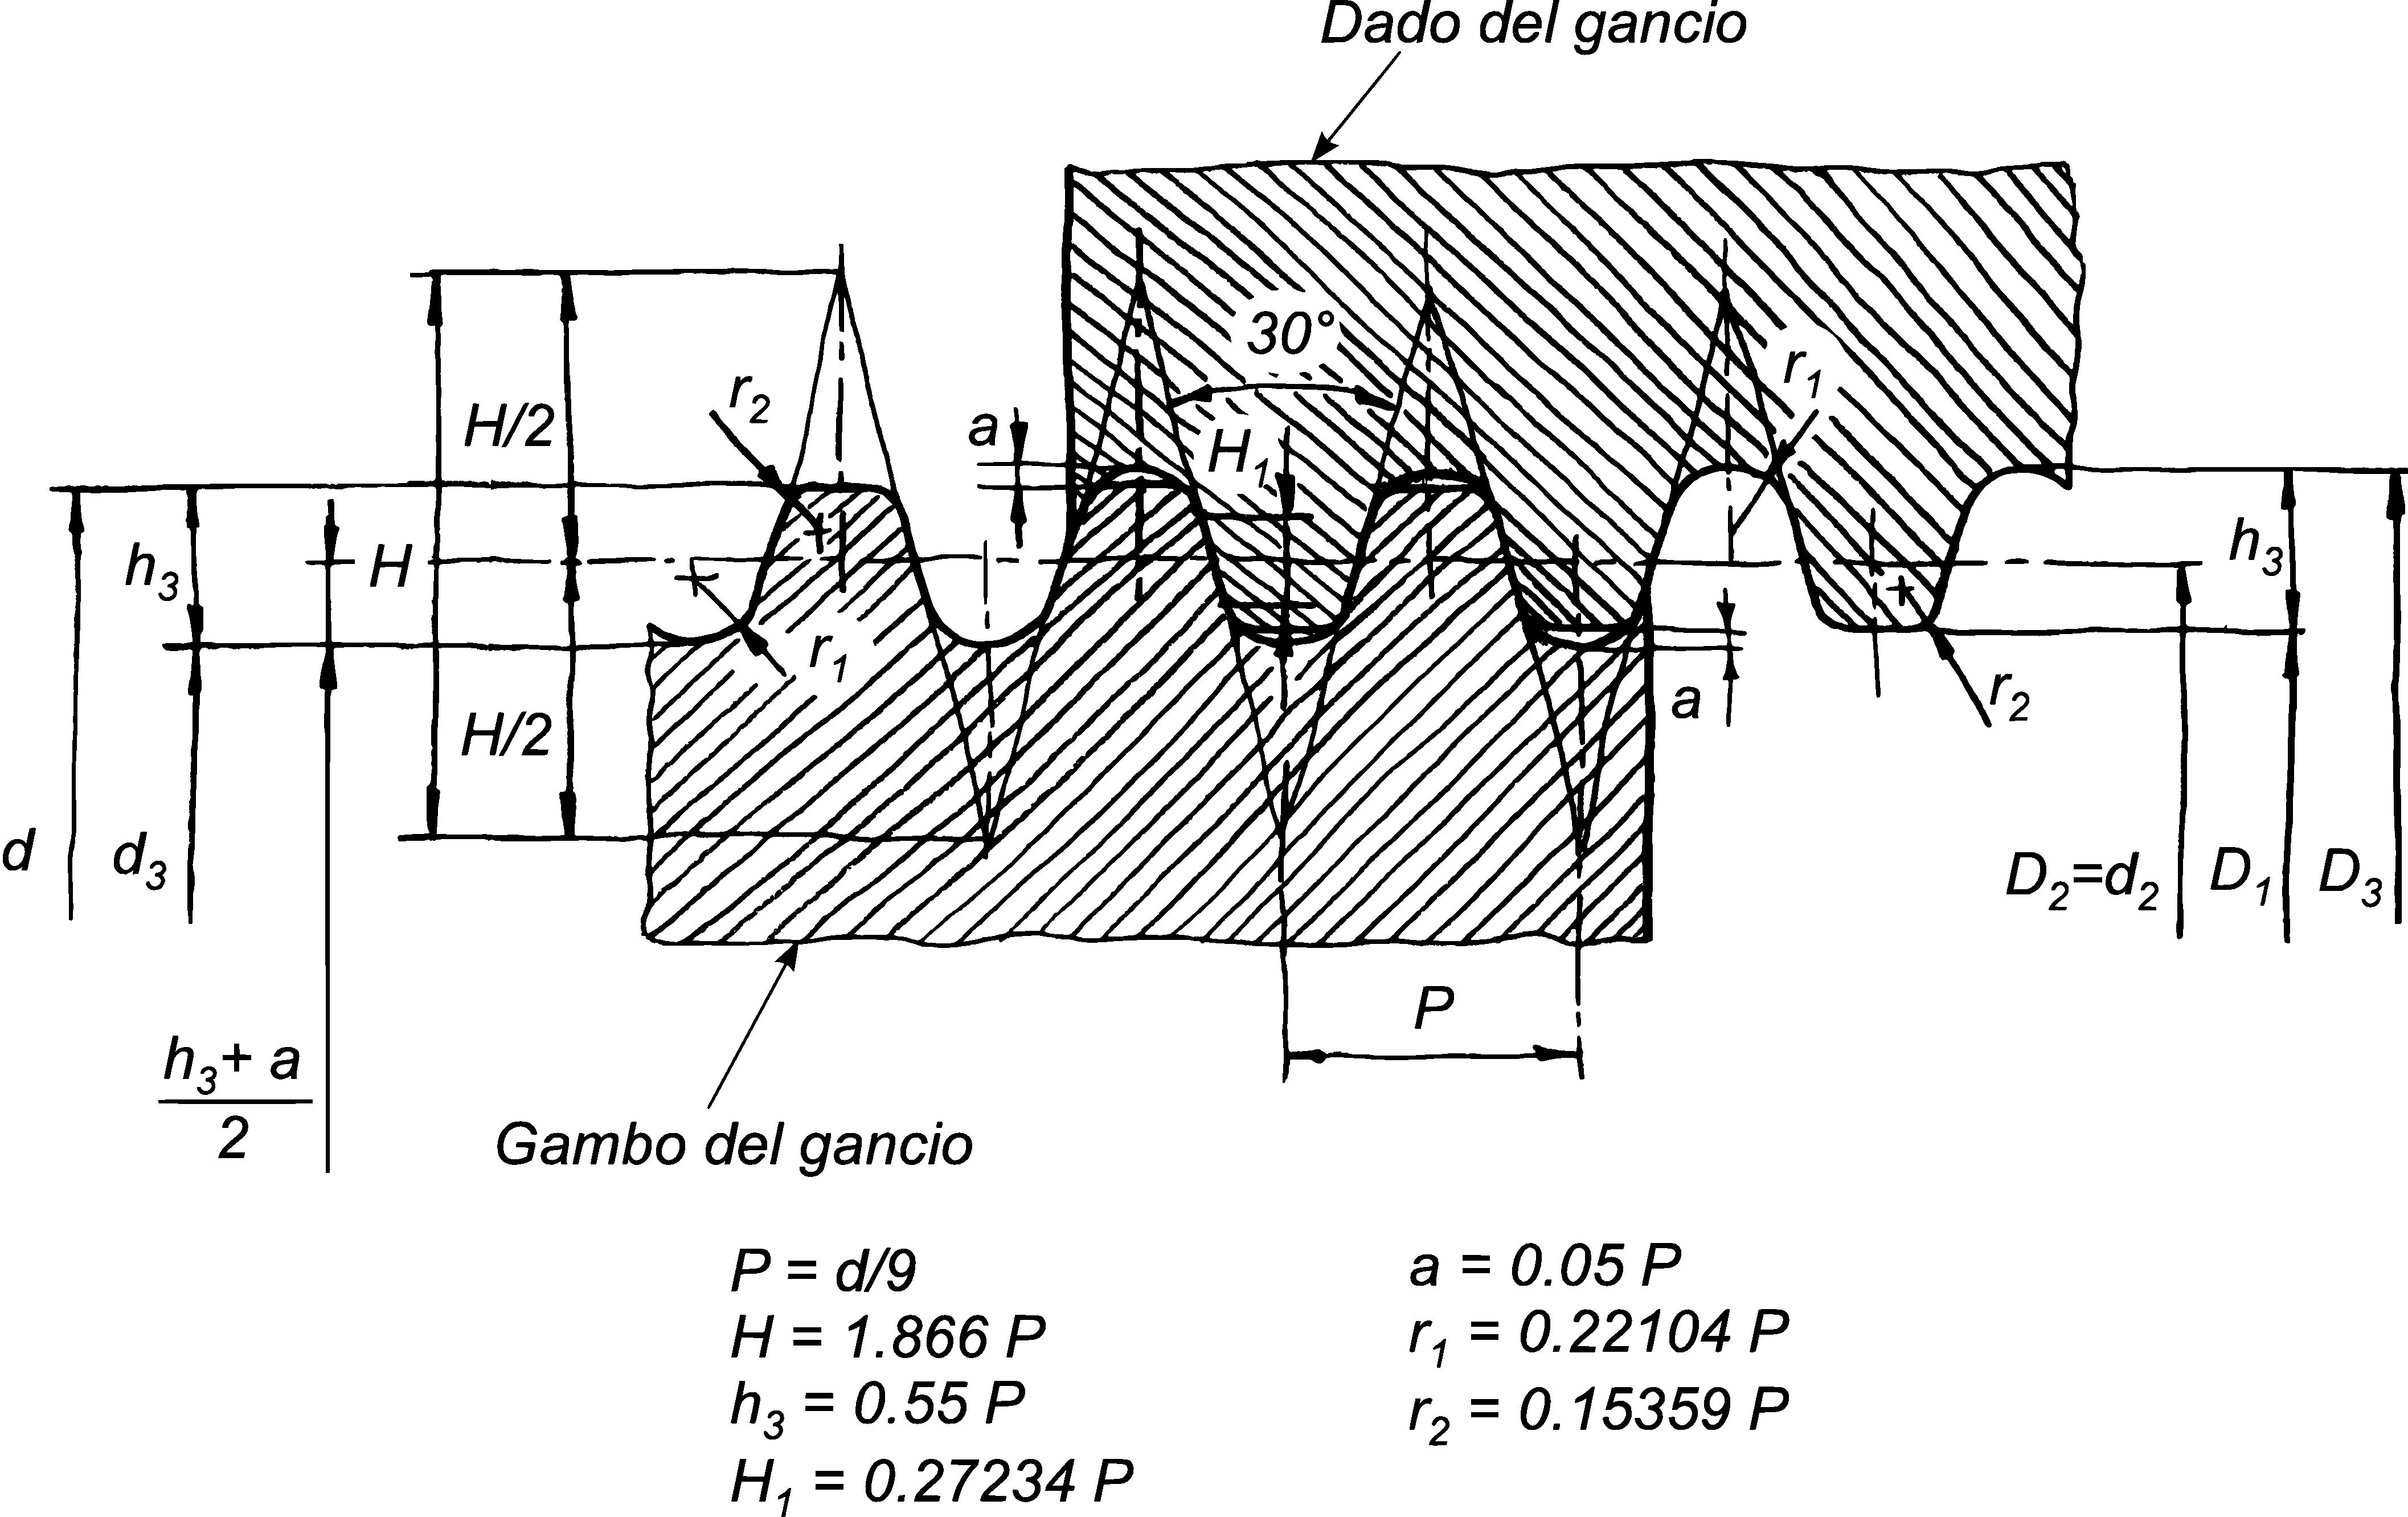
\includegraphics[width=.9\linewidth]{imgs/Cap5/5 FilDim}
  \captionof{figure}{Filettatura tonda UNI 9471 per ganci.}
  \label{fig:FilDim}
\end{minipage}%
\begin{minipage}{.45\textwidth}
  \centering
  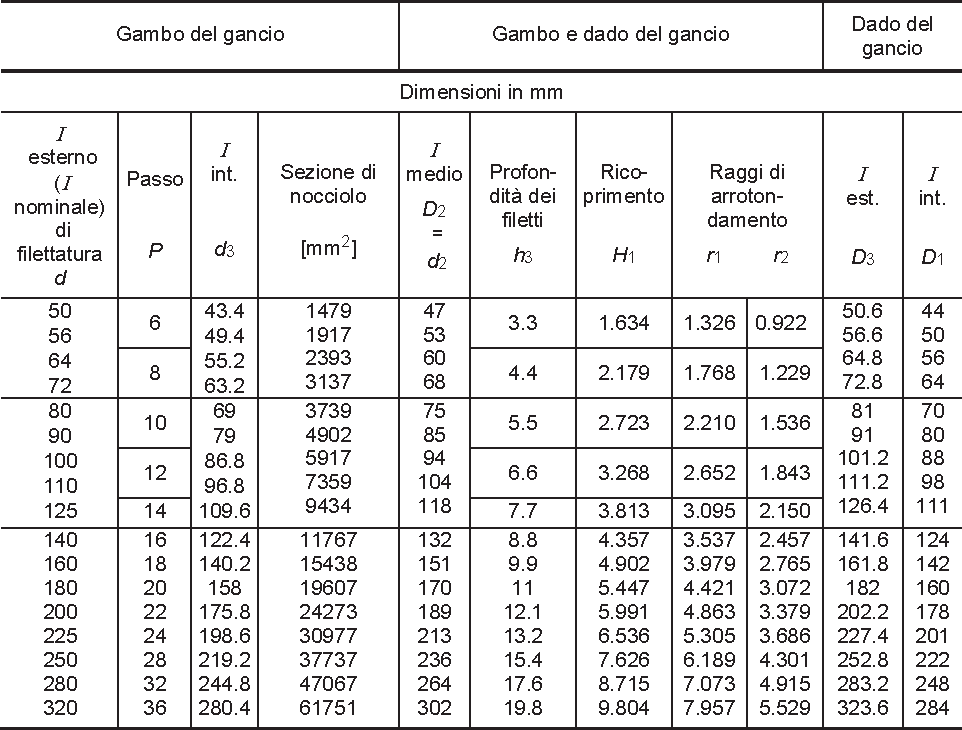
\includegraphics[width=.9\linewidth]{imgs/FilettaturaTabella}
  \captionof{figure}{Dimensioni filettatura tonda UNI 9471.}
  \label{fig:FilettaturaTabella}
\end{minipage}
\end{figure}

\subsection{Dimensionamento delle carrucole}
Le carrucole si differenziano in base al diametro della fune e al tipo di cuscinetto scelto. La fune, quando inserita nella puleggia, non toccherà il fondo ma sarà in contatto con i fianchi laterali della gola, questo viene fatto al fine di allungare la vita della fune. Per il dimensionamento si fa riferimento ai seguenti schizzi e alle annesse tabelle in figura \ref{fig:CarrTab1} e \ref{fig:CarrTab2}. 
\begin{figure}[H]
\centering
\begin{minipage}{.55\textwidth}
  \centering
  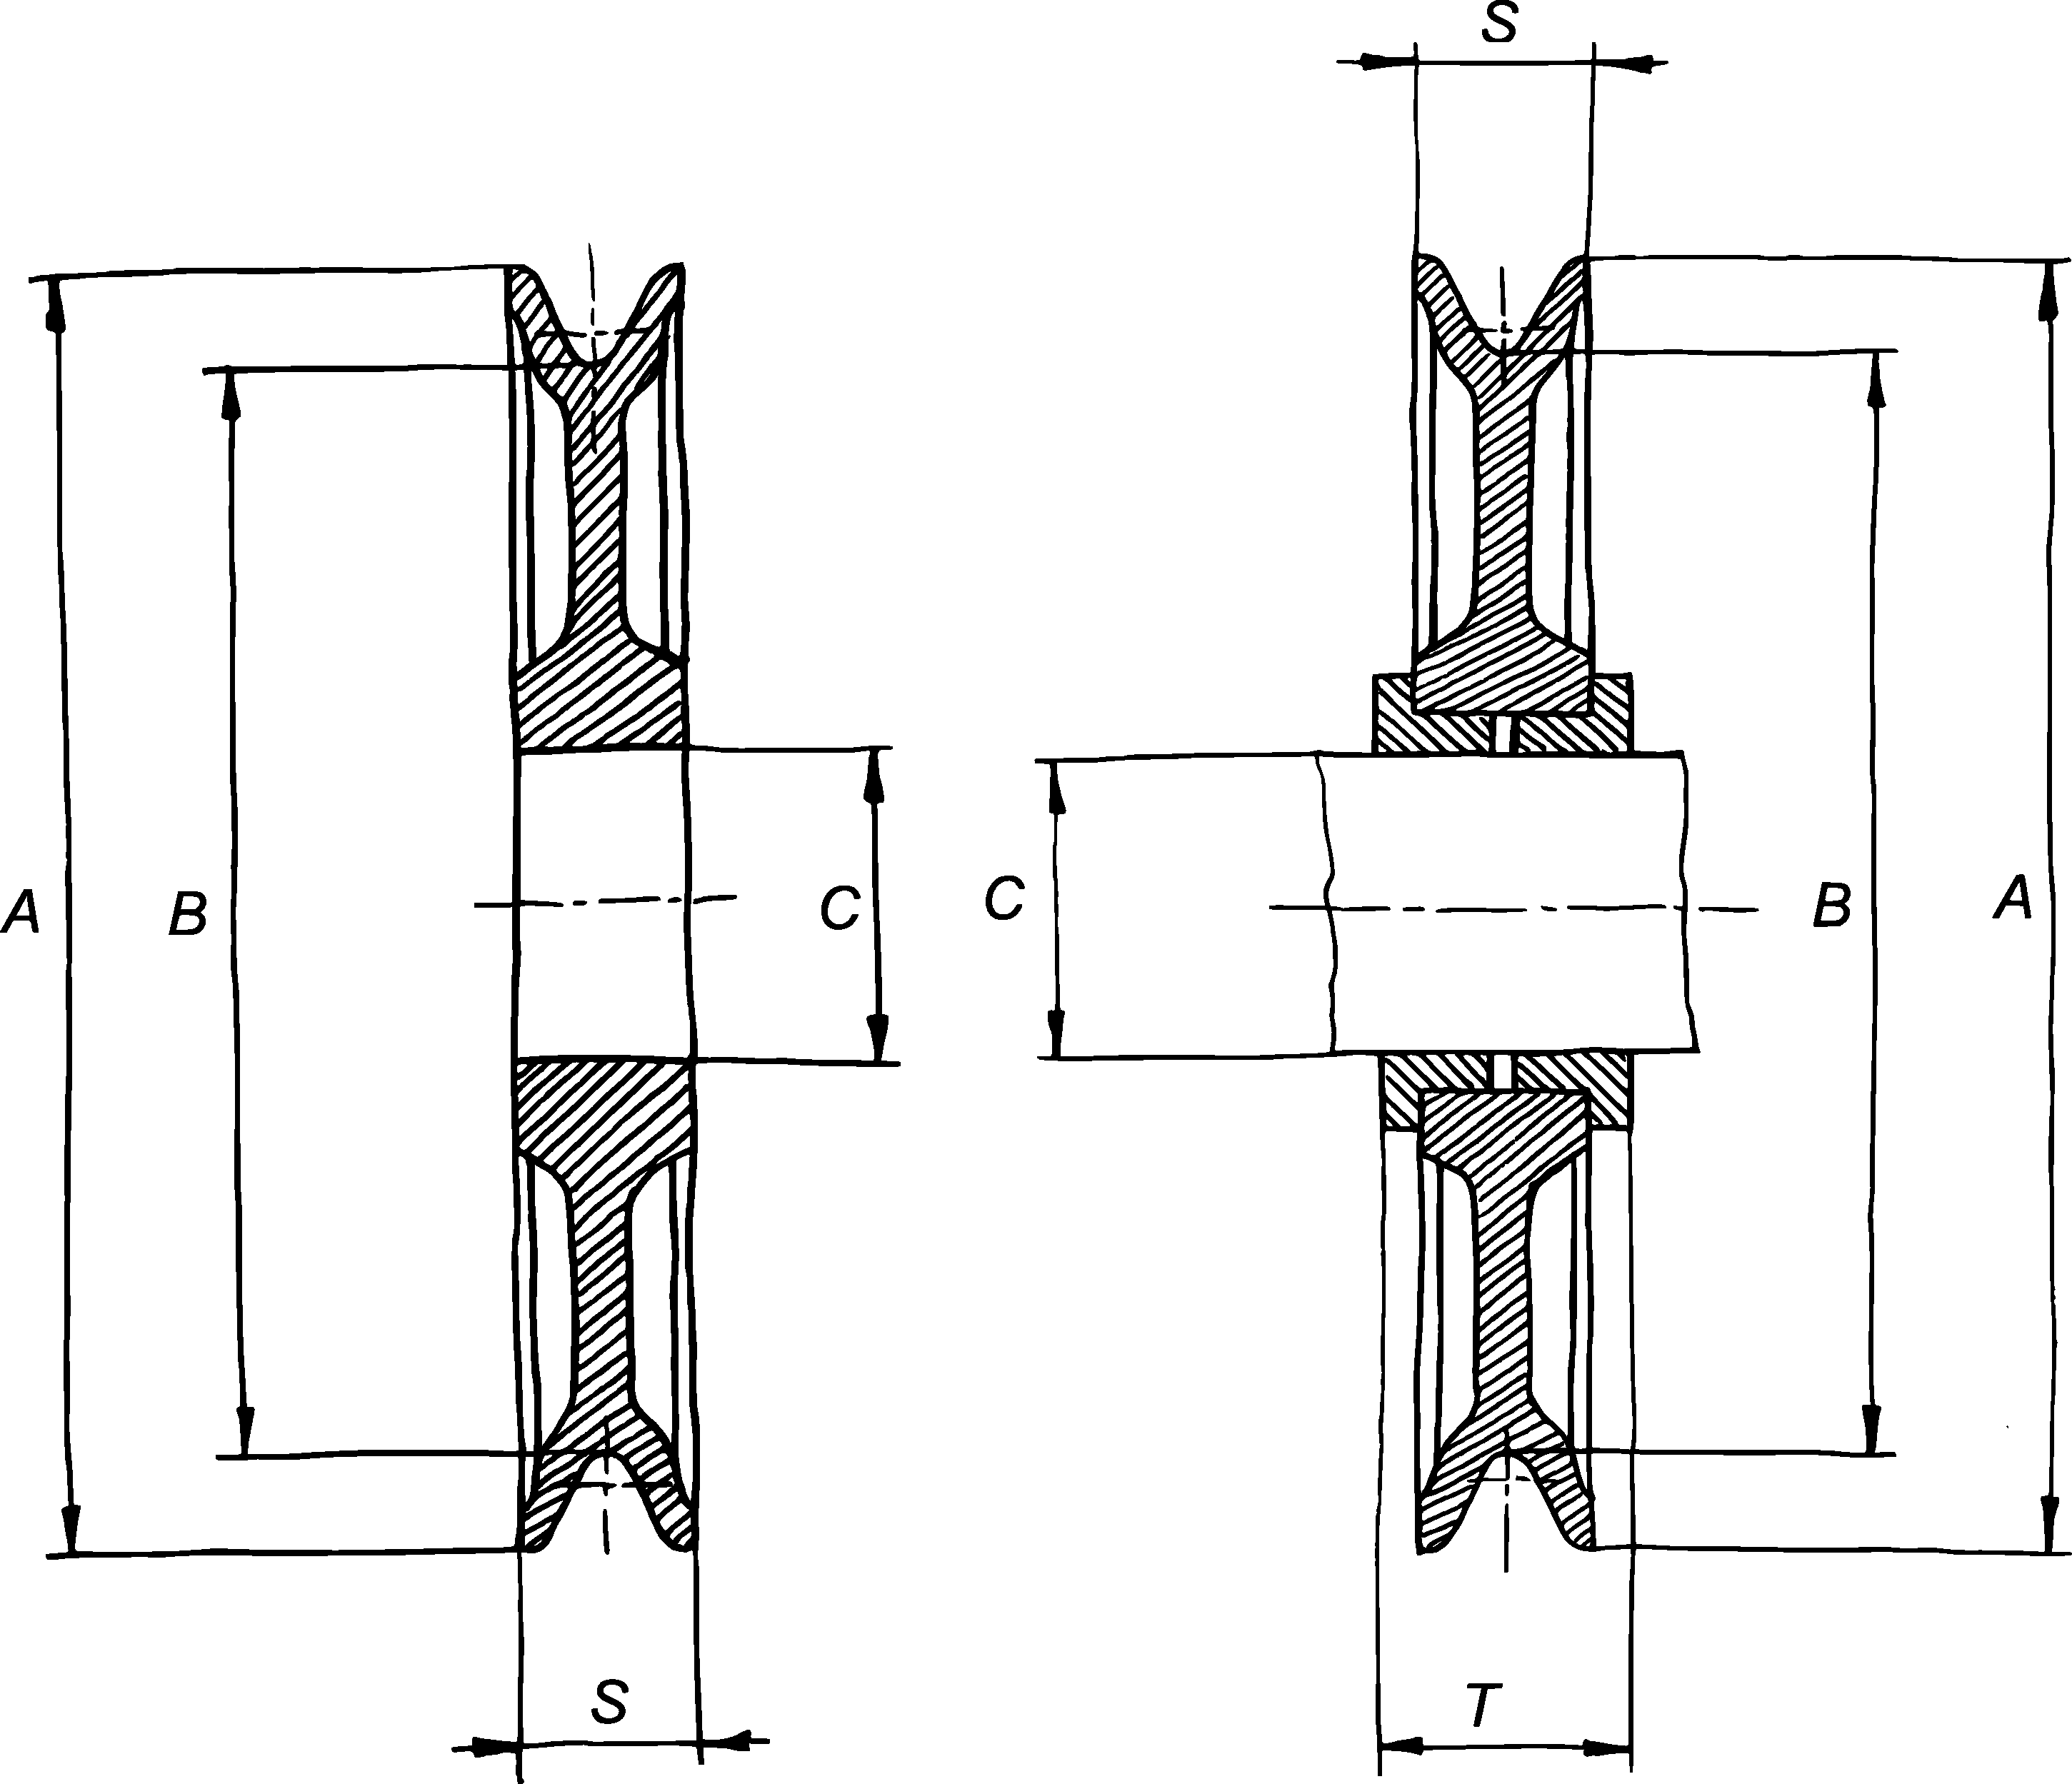
\includegraphics[width=.9\linewidth]{imgs/Carr1}
  \captionof{figure}{}
  \label{fig:Carr1}
\end{minipage}%
\begin{minipage}{.35\textwidth}
  \centering
  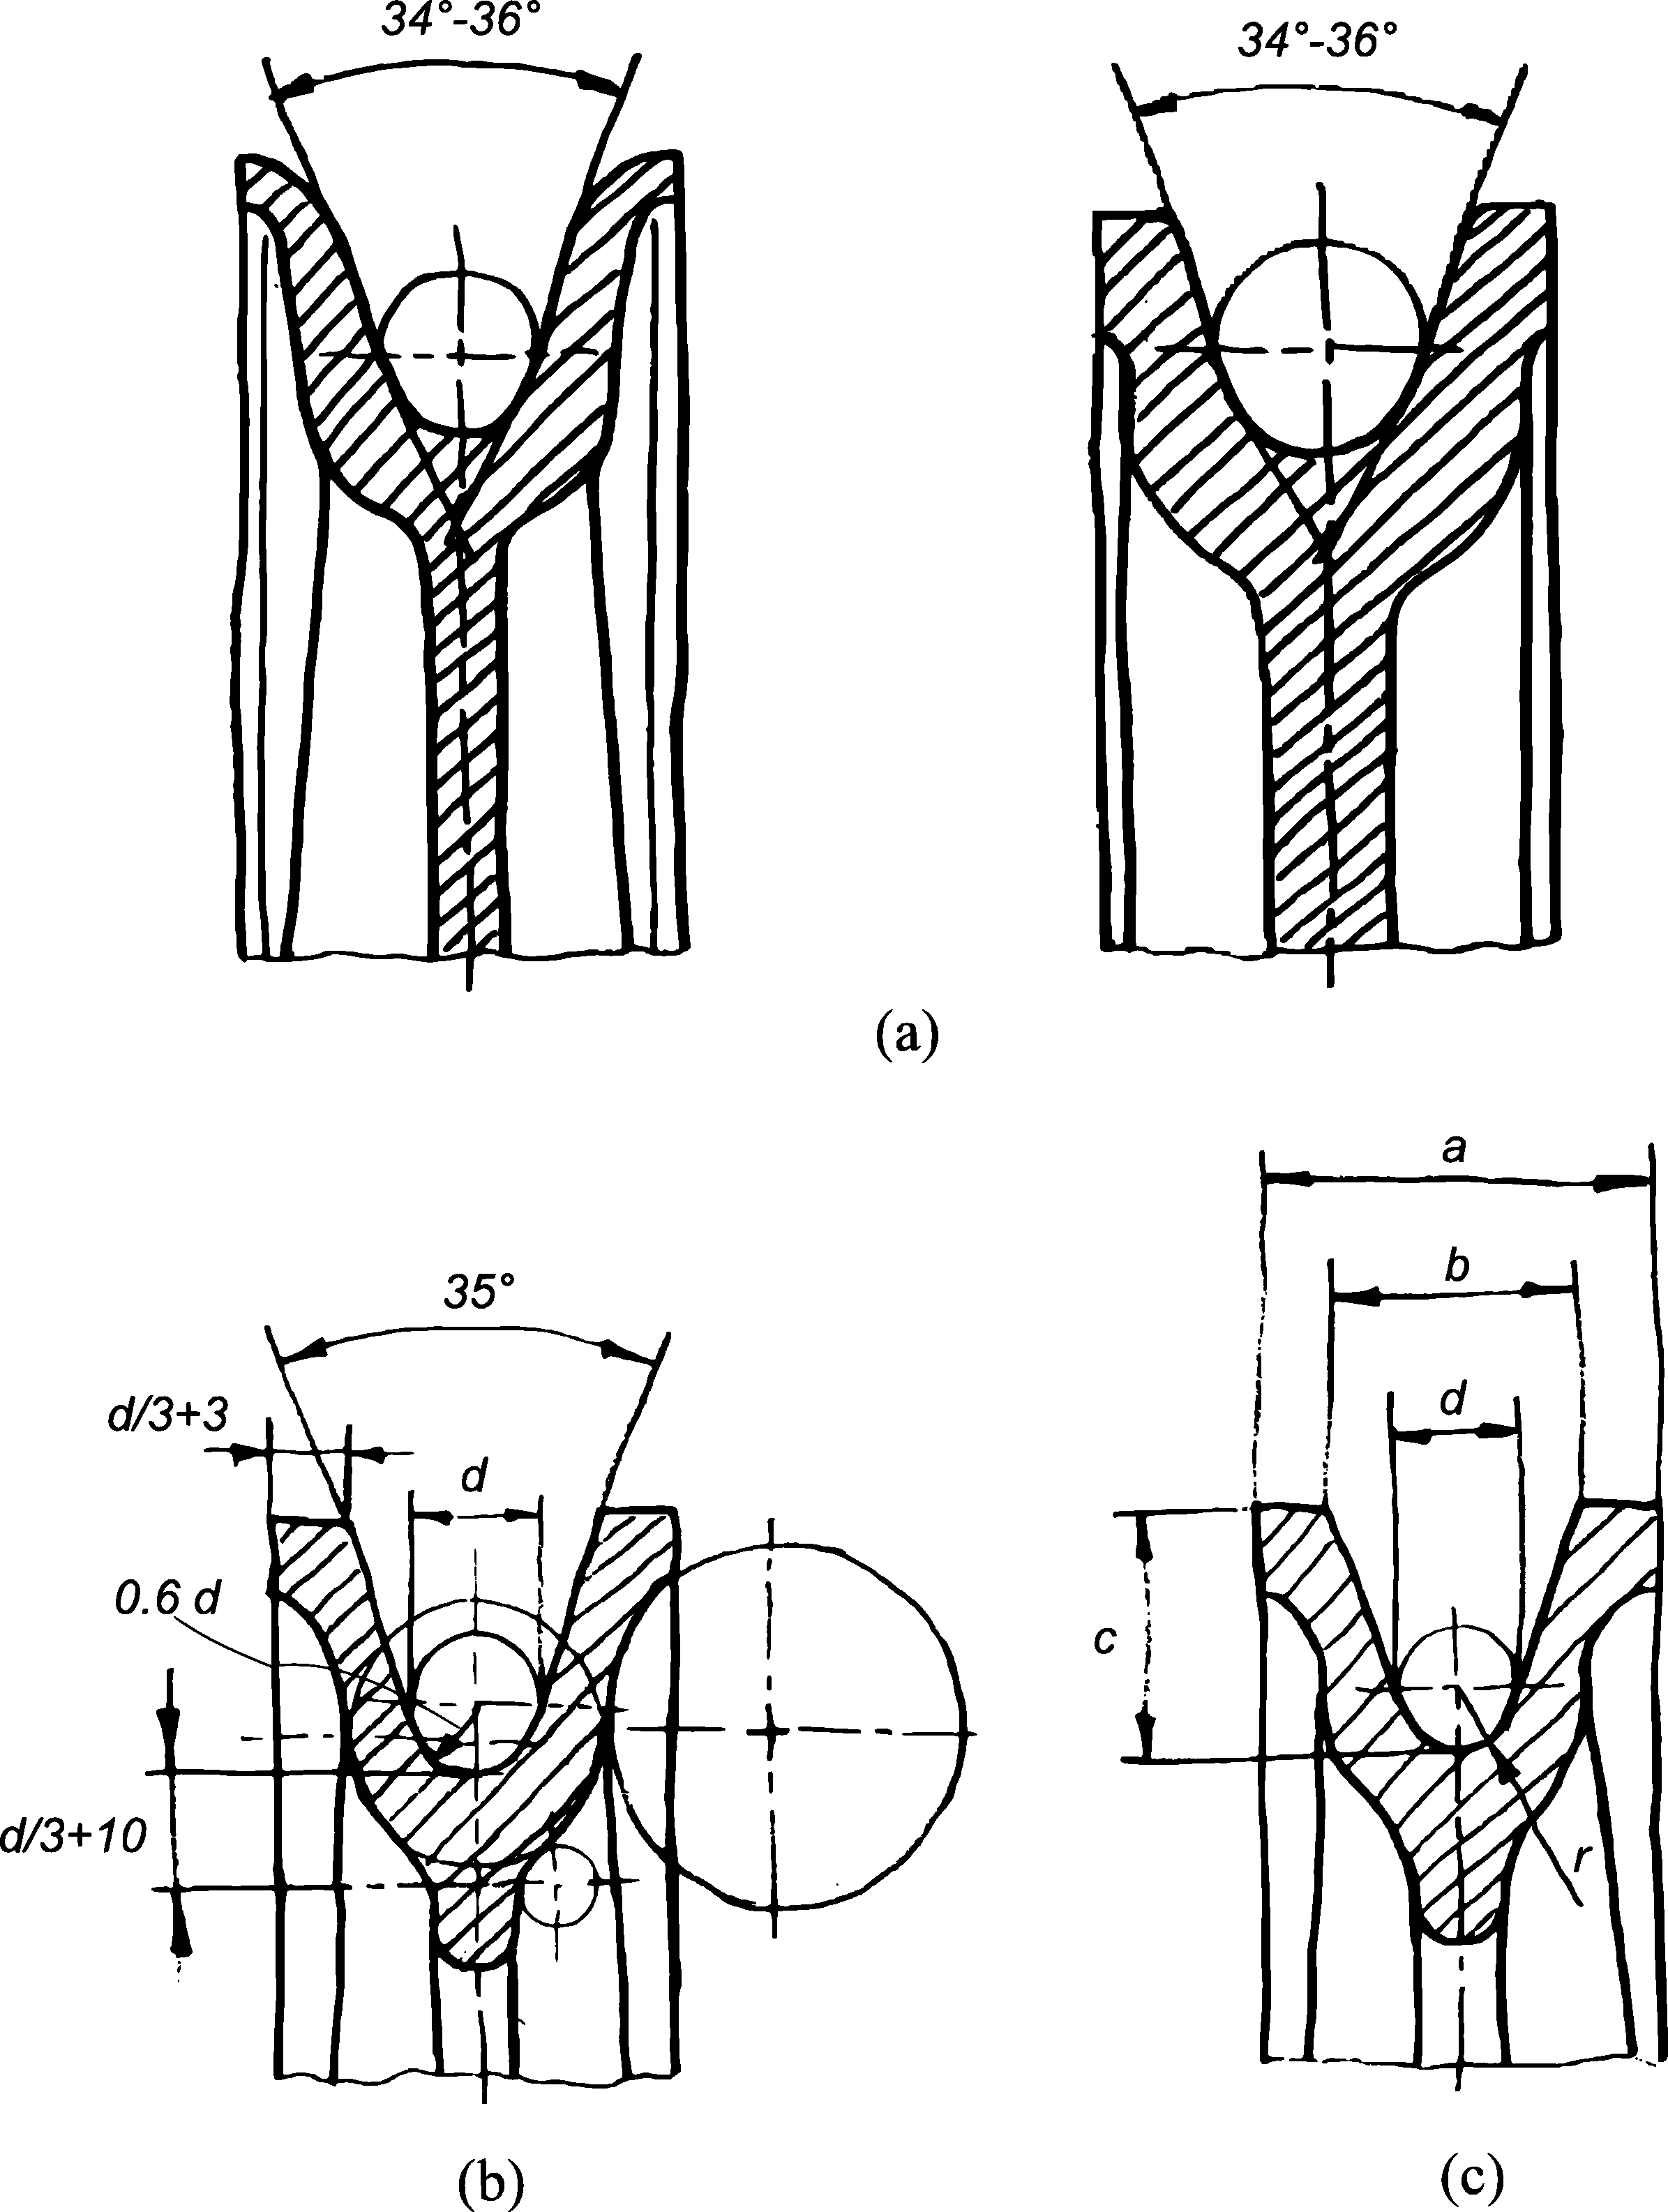
\includegraphics[width=.9\linewidth]{imgs/Carr2}
  \captionof{figure}{}
  \label{fig:Carr2}
\end{minipage}
\end{figure}

\begin{figure}[H]
\centering
  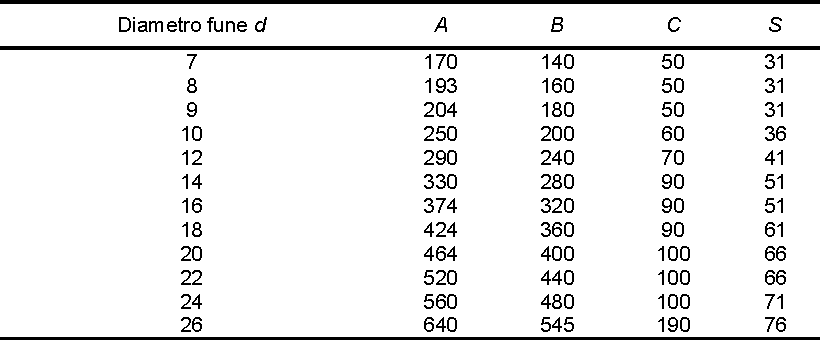
\includegraphics[width=.6\textwidth]{imgs/CarrTab1}
\caption{}
\label{fig:CarrTab1}
\end{figure}
\begin{figure}[H]
\centering
  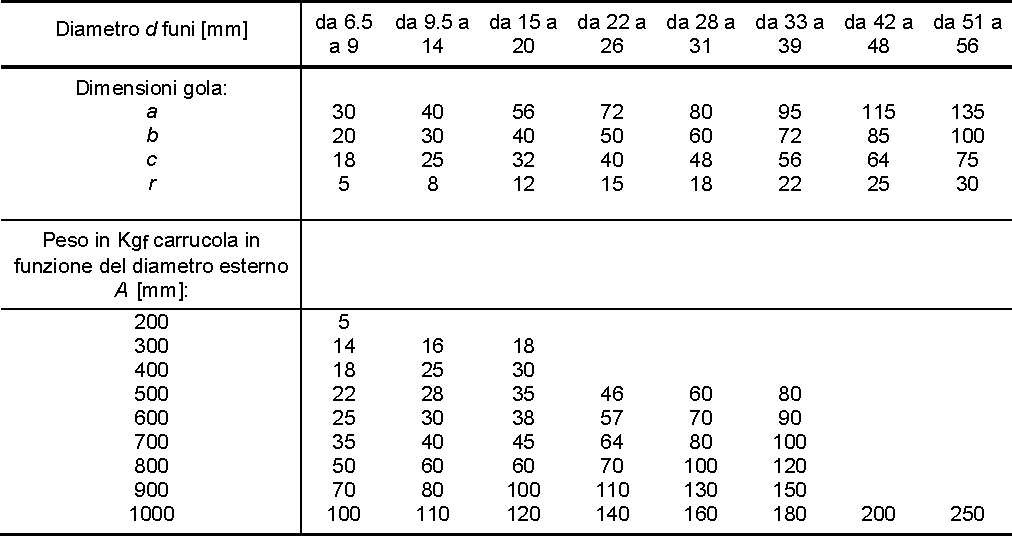
\includegraphics[width=.6\textwidth]{imgs/CarrTab2}
\caption{}
\label{fig:CarrTab2}
\end{figure}

\begin{table}[H]
\centering
\begin{tabular}{cccccccccc}
\toprule
\begin{tabular}[c]{@{}c@{}}d\\ $[mm]$\end{tabular} & \begin{tabular}[c]{@{}c@{}}A \\ $[mm]$\end{tabular} & \begin{tabular}[c]{@{}c@{}}B\\ $[mm]$\end{tabular} & \begin{tabular}[c]{@{}c@{}}C\\ $[mm]$\end{tabular} & \begin{tabular}[c]{@{}c@{}}T\\ $[mm]$\end{tabular} & \begin{tabular}[c]{@{}c@{}}S\\ $[mm]$\end{tabular} & \begin{tabular}[c]{@{}c@{}}a\\ $[mm]$\end{tabular} & \begin{tabular}[c]{@{}c@{}}b\\ $[mm]$\end{tabular} & \begin{tabular}[c]{@{}c@{}}c\\ $[mm]$\end{tabular} & \begin{tabular}[c]{@{}c@{}}r\\ $[mm]$\end{tabular} \\
\midrule
26                                                 & 640                                                 & 545                                                & 190                                                & 84                                                 & 76                                                 & 75                                                 & 50                                                 & 40                                                 & 15           \\
\bottomrule                                     
\end{tabular}
\caption{Valori di dimensionamento preliminare per le carrucole.}
\label{tab:CarrTabVal}
\end{table}
\subsection{Verifica dei becchi}
Come si vede dai calcoli, nel carico strutturale nominale sono stati considerati i contributi delle forze di inerzia dovute all'accelerazione del gancio in fase di salita e discesa nella movimentazione. Si è dimostrato che questo contributo è del tutto trascurabile, vale infatti per lo $0.4\%$ del carico totale. 

Procedendo con la verifica dei becchi sono state effettuate delle semplificazioni di calcolo: viene considerata una sezione trapezia di basi $a$ , $b$ e altezza $I_c$. Il valore dell'altezza dipende dalla posizione angolare della sezione in esame. Si individua la sezione del becco più sollecitata e si verifica che la sollecitazione massima che si instaura in tale sezione è inferiore alla massima ammissibile.

A questo punto si possono riportare le quote del dimensionamento preliminare ricavate dalle tabelle (vedi tabelle \ref{tab:interp_dimgen2}, \ref{tab:interp_dimgambo}).
\begin{table}[H]
\centering
\begin{tabular}{ccccccccc}
\toprule
\begin{tabular}[c]{@{}c@{}}$d_1$\\ $[mm]$\end{tabular} & \begin{tabular}[c]{@{}c@{}}$d$\\ $[mm]$\end{tabular} & \begin{tabular}[c]{@{}c@{}}$a$\\ $[mm]$\end{tabular} & \begin{tabular}[c]{@{}c@{}}$b$\\ $[mm]$\end{tabular} & \begin{tabular}[c]{@{}c@{}}$e$\\ $[mm]$\end{tabular} & \begin{tabular}[c]{@{}c@{}}$m$\\ $[mm]$\end{tabular} & \begin{tabular}[c]{@{}c@{}}$r$\\ $[mm]$\end{tabular} & \begin{tabular}[c]{@{}c@{}}$h$\\ $[mm]$\end{tabular} & \begin{tabular}[c]{@{}c@{}}$e_1$\\ $[mm]$\end{tabular} \\
\midrule
$207$                                             & $165$                                           & $145$                                           & $52$                                            & $166$                                           & $807$                                           & $269$                                           & $321$                                           & $372$              \\
\bottomrule                              
\end{tabular}
\caption{Interpolazione dei dati in tabella \ref{fig:DimGen2}.}
\label{tab:interp_dimgen2}
\end{table}


\begin{table}[H]
\centering
\resizebox{\textwidth}{!}{\begin{tabular}{ccccccccccccc}
\toprule
\begin{tabular}[c]{@{}c@{}}$d_1$\\ $[mm]$\end{tabular} & \begin{tabular}[c]{@{}c@{}}$d_5$\\ $[mm]$\end{tabular} & \begin{tabular}[c]{@{}c@{}}$d$\\ $[mm]$\end{tabular} & \begin{tabular}[c]{@{}c@{}}$d_4$\\ $[mm]$\end{tabular} & \begin{tabular}[c]{@{}c@{}}$d_3$\\ $[mm]$\end{tabular} & \begin{tabular}[c]{@{}c@{}}$d_6$\\ $[mm]$\end{tabular} & \begin{tabular}[c]{@{}c@{}}$I_3$\\ $[mm]$\end{tabular} & \begin{tabular}[c]{@{}c@{}}$m$\\ $[mm]$\end{tabular} & \begin{tabular}[c]{@{}c@{}}$n$\\ $[mm]$\end{tabular} & \begin{tabular}[c]{@{}c@{}}$p$\\ $[mm]$\end{tabular} & \begin{tabular}[c]{@{}c@{}}$r_9$\\ $[mm]$\end{tabular} & \begin{tabular}[c]{@{}c@{}}$r_{10}$\\ $[mm]$\end{tabular} & \begin{tabular}[c]{@{}c@{}}$r_{11}$\\ $[mm]$\end{tabular} \\
\midrule
$170$                                              & $140$                                              & $FT140 \times 16$                                       & $120$                                              & $122.4$                                            & $90$                                               & $280$                                              & $125$                                            & $50$                                             & $12$                                             & $10$                                               & $40$                                                & $5$                                                \\
\bottomrule
\end{tabular}}
\caption{Interpolazione dei dati in tabella \ref{fig:DimGambo}.}
\label{tab:interp_dimgambo}
\end{table}


Per effettuare i calcoli si utilizza il software \textit{Mathcad}.
Come modelli matematici si userà la teoria dei solidi a grande curvatura, questa comporta però diversi problemi:
\begin{itemize}
\item La sezione resistente non è costante al variare dell'angolo $\psi$ compreso tra il segmento $AD$ e la verticale;
\item La curva descritta dal baricentro delle singole sezioni resistenti al variare di tale angolo ha un raggio di curvatura variabile;
\item Il centro di curvatura varia passando da un baricentro all'altro;
\item Non si riesce a determinare in maniera univoca un'unica curva dei baricentri delle sezioni resistenti;
\item La traccia della sezione resistente o il suo prolungamento non passa per il centro di curvatura corrispondente al baricentro della sezione stessa.
\end{itemize}

La sezione resistente individuata dall'intersezione del becco con un piano passante per i punti $A$ e $D$ avrebbe centro di curvatura non appartenente al prolungamento della traccia della sezione resistente. 
Per applicare la teoria dei solidi a grande curvatura viene introdotto un solido fittizio a grande curvatura, il cui centro di curvatura è passante per la retta d'azione del carico applicato. 
Il solido fittizio è individuato dalla linea tratteggiata $MNHI$ (figura \ref{fig:solidoFittizio}) e il centro di curvatura è individuato dal centro $O'$. 
Si considera la condizione di sollecitazione più critica, ovvero il carico (fune) inclinata di $45^\circ$ rispetto all'asse del gambo. 
Sul baricentro $L$ della sezione $HI$ sarà quindi applicato un carico pari a $2 \; Q/\sqrt{2}$. 
Si considera tale sezione trapezia con basi $a, \;b$ e altezza $I_r$.
La sezione $NM$ è quella più sollecitata in quanto è presente il massimo momento flettente.
\begin{figure}
\centering
\begin{minipage}{.63\textwidth}
  \centering
  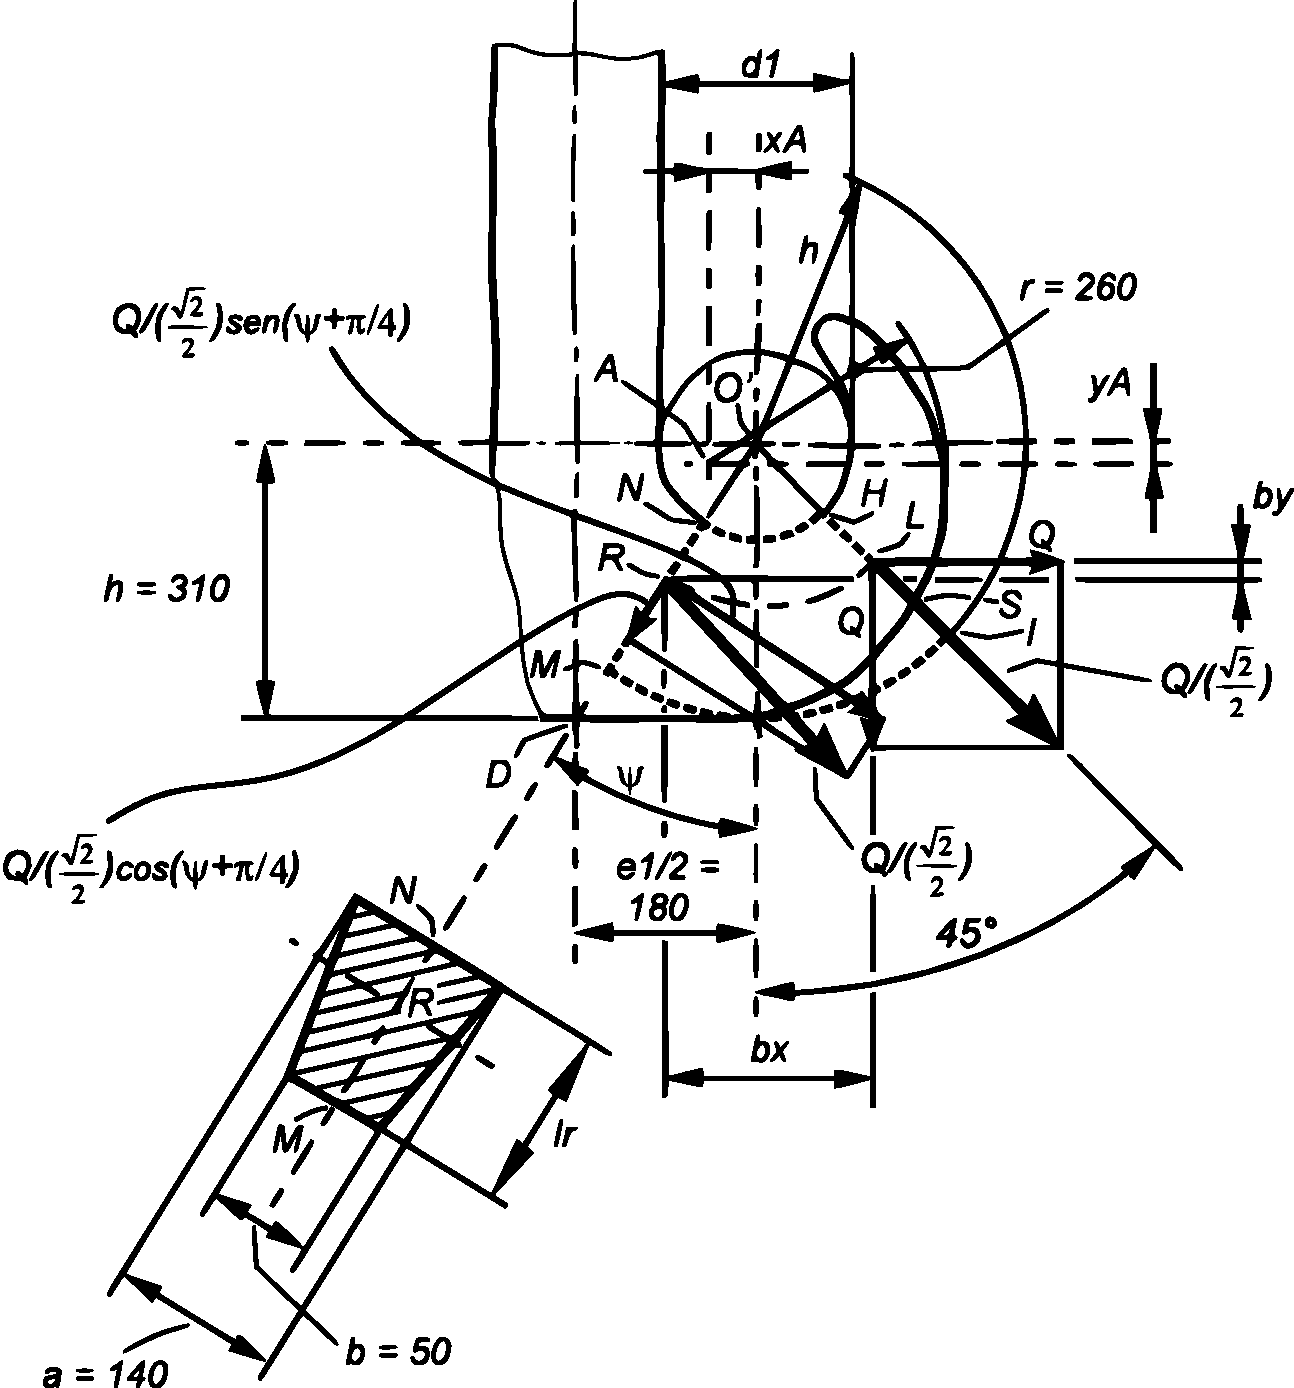
\includegraphics[width=.7\linewidth]{imgs/Cap5/92 SolidoFitt}
  \captionof{figure}{Solido fittizio per poter utilizzare la teoria dei solidi a grande curvatura.}
  \label{fig:solidoFittizio}
\end{minipage}%
\begin{minipage}{.33\textwidth}
  \centering
  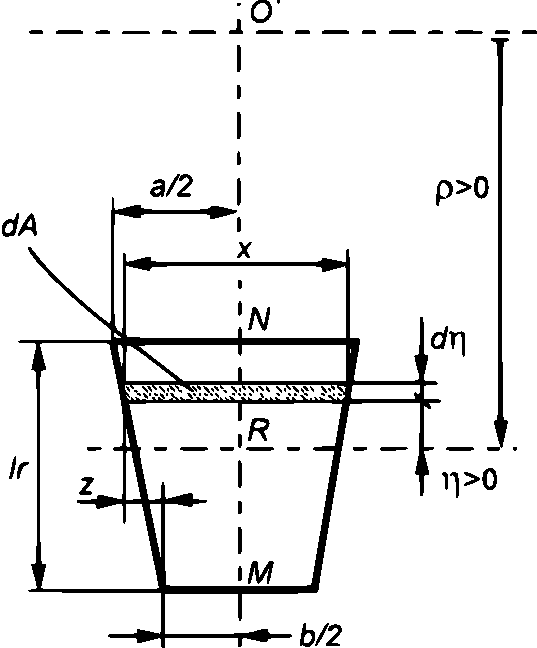
\includegraphics[width=.7\linewidth]{imgs/chiTrap}
  \captionof{figure}{Calcolo di $\chi$ per la sezione trapezia.}
  \label{fig:chiTrapezio}
\end{minipage}
\end{figure} 

\begin{figure}
\centering
  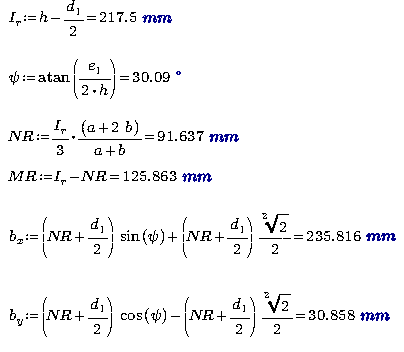
\includegraphics[width=.5\textwidth]{imgs/Mathcad1}
\caption{Calcoli strutturali relativi al primo solido fittizio.}
\label{fig:Mathcad1}
\end{figure}
\begin{figure}
\centering
  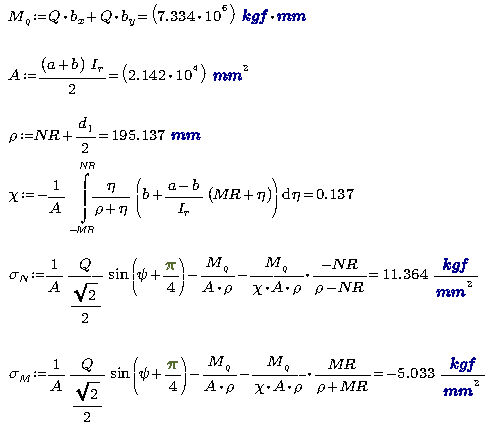
\includegraphics[width=.45\textwidth]{imgs/Mathcad2}
\caption{Calcoli strutturali relativi al primo solido fittizio, sforzo a flessione $\sigma$ agente nei punti $N$ e $M$.}
\label{fig:Mathcad2}
\end{figure}
\begin{figure}[H]
\centering
  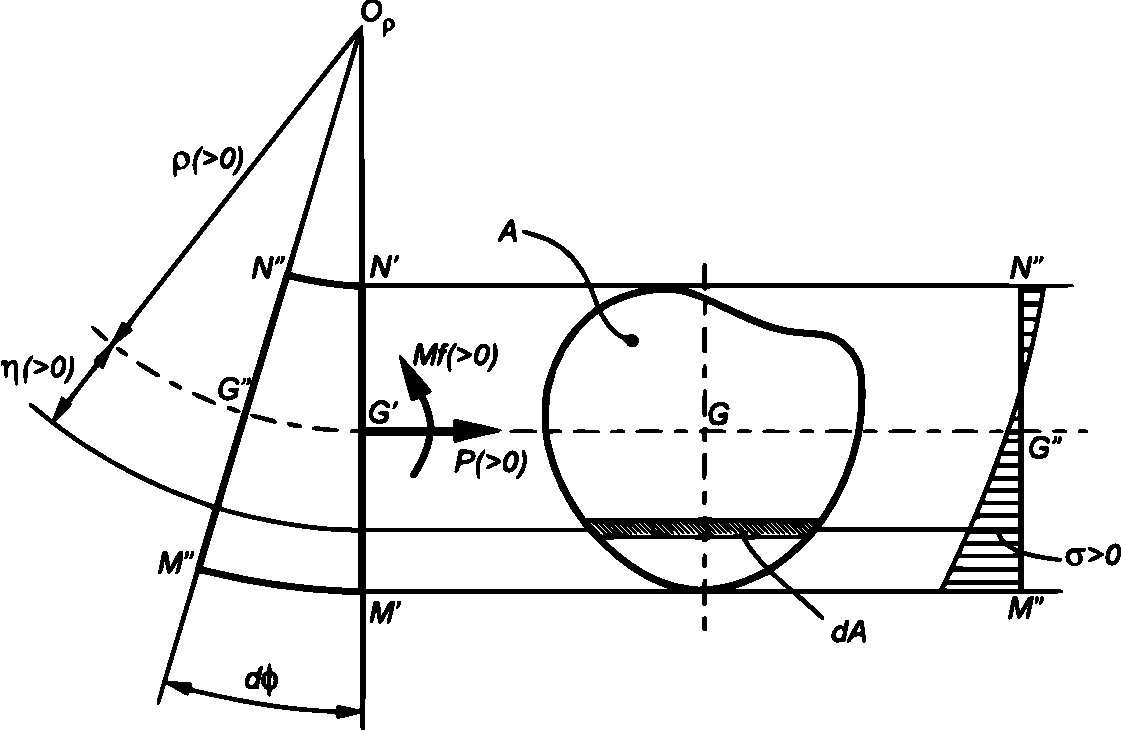
\includegraphics[width=.5\textwidth]{imgs/Cap5/94 ConcioGC}
\caption{Concio di trave.}
\label{fig:ConcioGC}
\end{figure}

Con $P$ si indica il carico normale alla sezione applicato sul baricentro della sezione stessa, $\rho$ è il raggio di curvatura baricentrico, $\eta$ è la distanza dell'area $dA$ dal baricentro $R$, misurata nella direzione di $\rho$ e $\chi$ è un fattore adimensionale che dipende dalla forma della geometria della sezione radiale del concio.
L'asse neutro non è più baricentrico e l'andamento delle tensioni non è più lineare come nel caso della trave rettilinea. 
L'andamento delle tensioni espresso dalla formula precedente si riferisce alle sezioni $N'M'$ e $N''M''$. 
La massima tensione di trazione è notevolmente inferiore al limite di snervamento considerando un acciaio avente un carico di snervamento di $350$ $MPa$.

Si valutano ora gli sforzi di taglio relativi alla sezione $ND$ (figura \ref{fig:Mathcad3}). 
Nel primo calcolo si considera la sezione rettangolare di lati $ND$ e $b$ e successivamente, in via cautelativa, si considera la sezione rettangolare di lati $I_r$ e $b$.
\begin{figure}[H]
\centering
  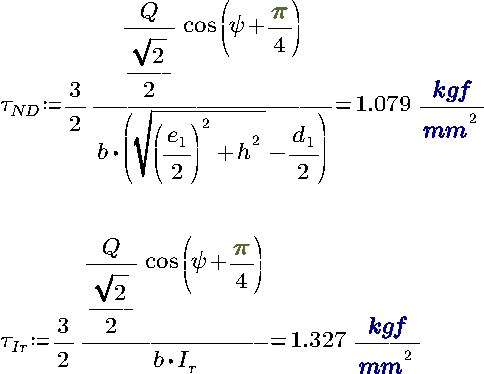
\includegraphics[width=.35\textwidth]{imgs/Mathcad3}
\caption{}
\label{fig:Mathcad3}
\end{figure}
Gli sforzi di taglio risultano essere trascurabili. 
Questi agiscono inoltre in corrispondenza del baricentro della sezione, vicino all'asse neutro, dove gli sforzi dovuti al momento flettente sono limitati.
Fino a questo punto si è sottostimata la resistenza della sezione $NM$, inferiore a quella reale $ND$, mentre si è sovrastimata la sezione $HI$ superiore a quela reale $HS$. 
\begin{figure}[H]
\centering
  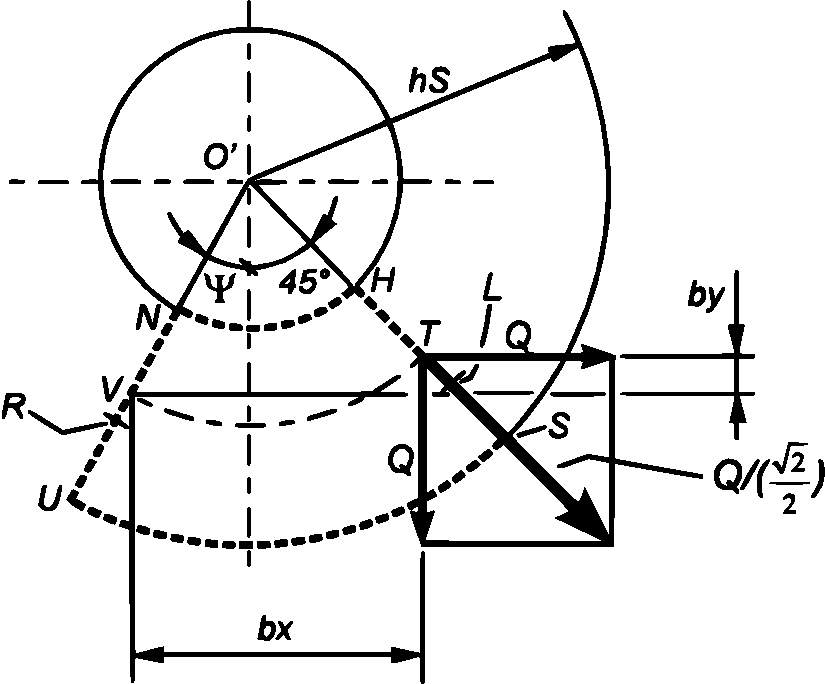
\includegraphics[width=.4\textwidth]{imgs/Cap5/95 SolidoFitt2}
\caption{Nuovo solido fittizio.}
\label{fig:SolidoFitt2}
\end{figure}
\begin{figure}[H]
\centering
  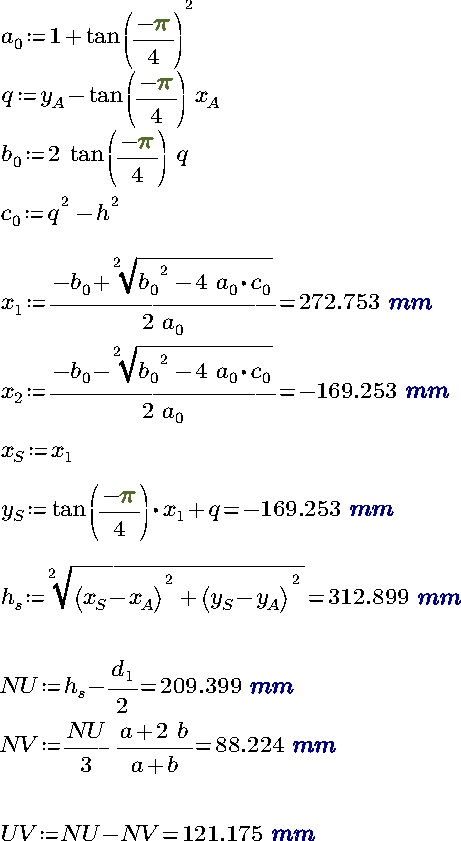
\includegraphics[width=.4\textwidth]{imgs/Mathcad4}
\caption{}
\label{fig:Mathcad4}
\end{figure}
\begin{figure}[H]
\centering
  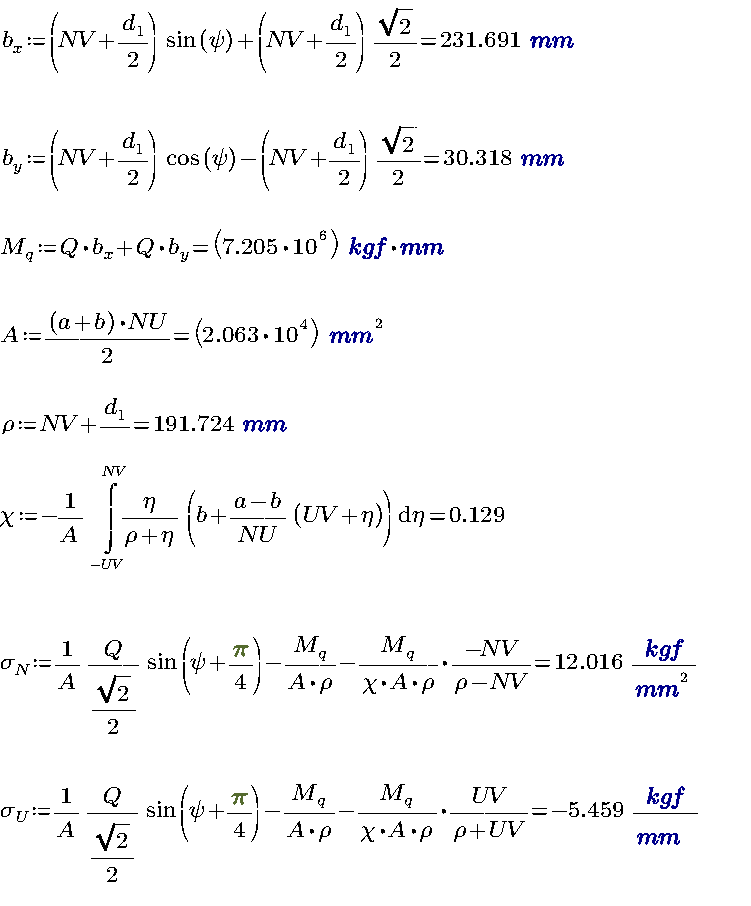
\includegraphics[width=.44\textwidth]{imgs/Mathcad5}
\caption{}
\label{fig:Mathcad5}
\end{figure}
Per eseguire i calcoli con maggior accuratezza si definisce un nuovo solido fittizio $UNHS$ di sezione costante pari ad $HS$. Il carico viene applicato nel baricentro $T$ della sezione considerata e si andranno a stimare le tensioni nei punti $N$ e $U$ (sezione maggiormente sollecitata).
Eseguendo i calcoli come è stato fatto per il solido fittizio precedente, si vanno a calcolare le sollecitazioni nei punti $N$ e $U$, rispettivamente a trazione e a compressione.

Tali valori risultano accettabili in base al limite di snervamento a cui è stato fatto riferimento. 
\clearpage
\subsection{Verifica del gambo}

\begin{figure}[H]
\centering
\begin{minipage}{.47\textwidth}
  \centering
  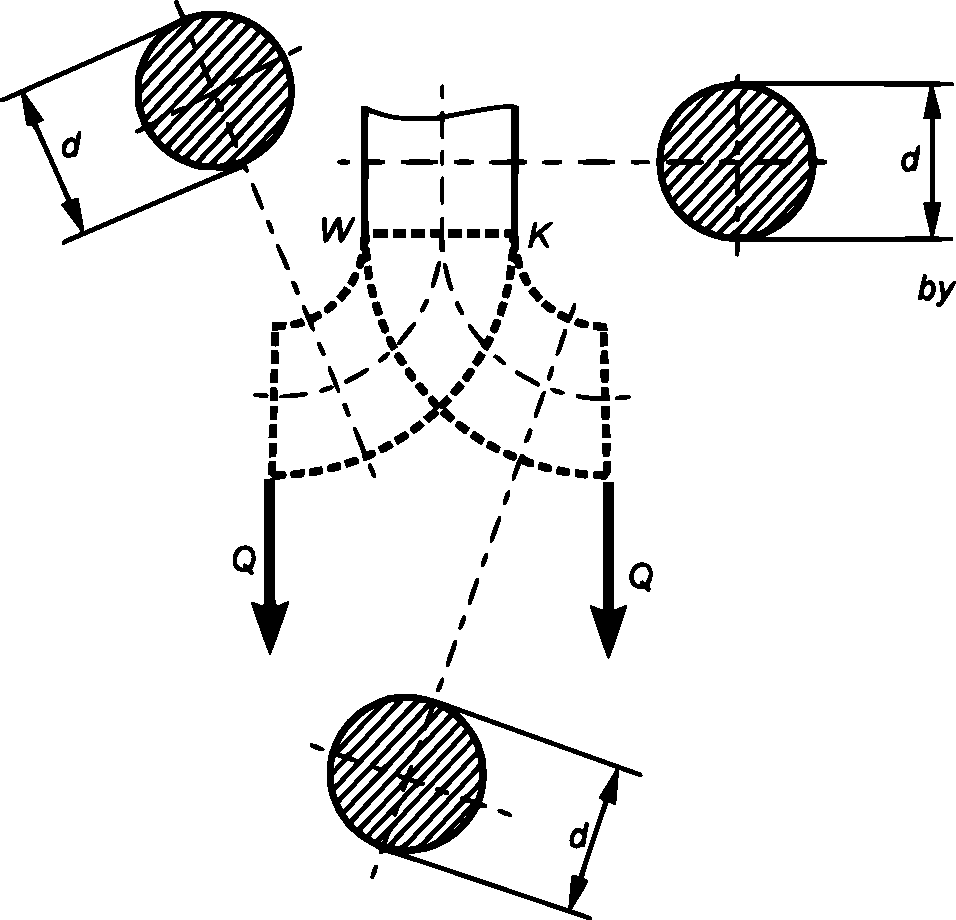
\includegraphics[width=.9\linewidth]{imgs/Cap5/96 SolidoFitt3}
  \captionof{figure}{Solido fittizio relativo al gambo del gancio.}
  \label{fig:Carr1}
\end{minipage}%
\begin{minipage}{.47\textwidth}
  \centering
  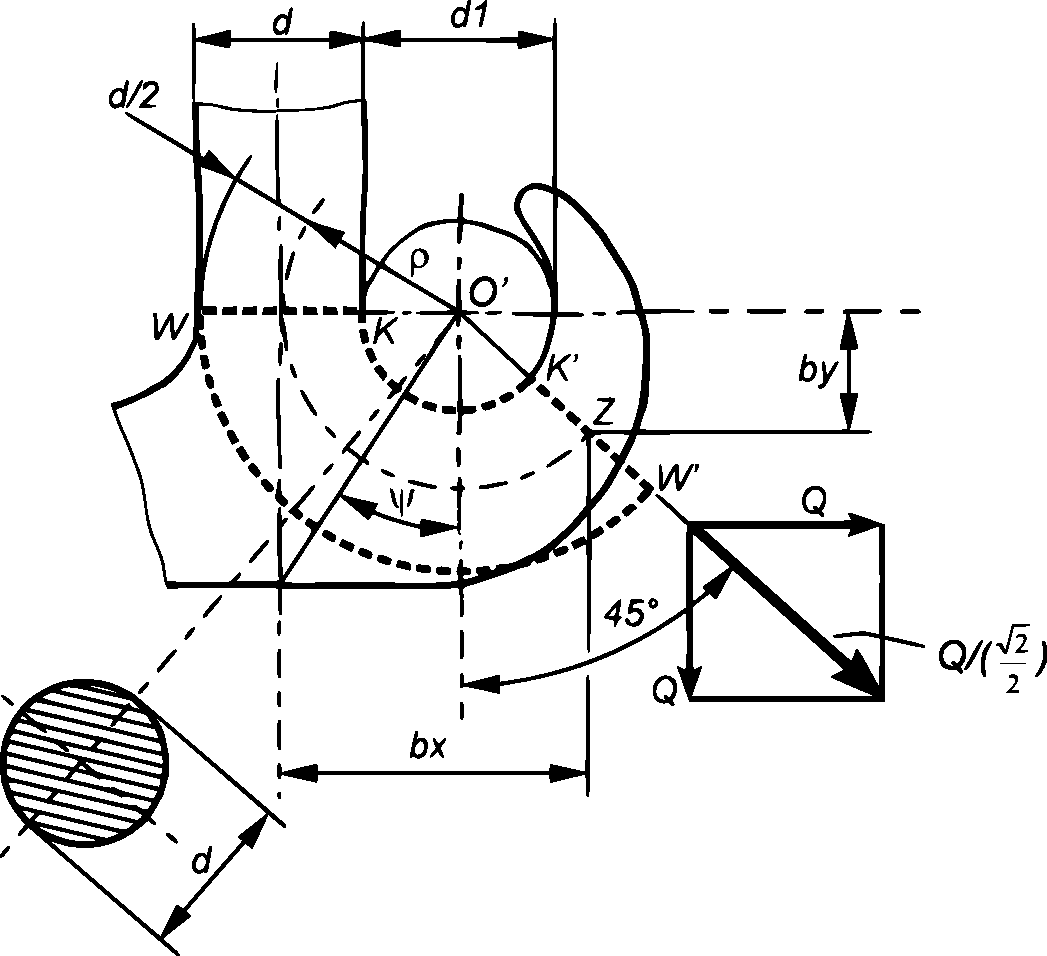
\includegraphics[width=.9\linewidth]{imgs/Cap5/SolidoFittGambo}
  \captionof{figure}{Schema di carico del nuovo solido fittizio.}
  \label{fig:Carr2}
\end{minipage}
\end{figure}
Si vuole ora stimare la sollecitazione che si instaura nel gambo. 
Si definisce un nuovo solido fittizio come prolungamento della sezione $WK$ e con carico applicato in corrispondenza del baricentro $Z$ della sezione $K'W'$.
Si considera la condizione di carico simmetrico e si effettua quindi la sovrapposizione degli effetti nel punto $K$ rispetto ai carichi agenti su entrambi i becchi. 
Lo sforzo agente reale è dato dalla somma algebrica delle sollecitazioni $\sigma_K$ e $\sigma_W$, una a trazione e una a compressione. Il valore ottenuto è da considerarsi accettabile.
\begin{figure}[H]
\centering
  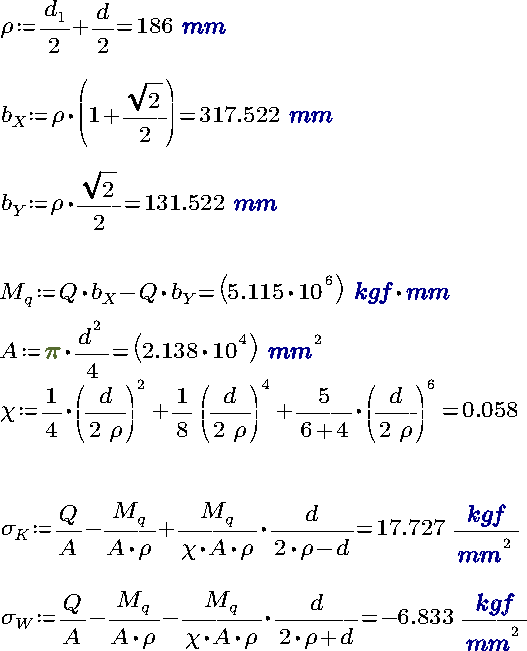
\includegraphics[width=.4\textwidth]{imgs/Mathcad6}
\caption{}
\label{fig:Mathcad6}
\end{figure}
In ultimo devono essere fatte delle considerazioni per quanto riguarda il gambo del gancio.
Si consideri il carico $Q$ applicato verticalmente con retta d'azione passante per il centro $O'$ e si calcoli il momento flettente $M_q$.
Il valore qui ricavato è identico al precedente dalcolato con carico posto a $45^\circ$, questo è dato dal fatto che il raggio di curvatura $\rho$ è costante; in questo modo restano invariate anche $\sigma_K$ e $\sigma_W$.

Per la verifica della parte superiore del gambo si procede considerando una sollecitazione assiale con un carico pari alla portata nominale.
Si calcolano il numero di filetti in presa $i$. Con $P$ viene indicato il passo della filettatura e con $m$ la lunghezza della parte filettata.

Nel calcolo si utilizza un coefficiente correttivo pari a $0.8$ in quanto filetti iniziali e finali non sono coinvolti nella presa. 
Per stimare il peso del gancio si fa riferimento alle tabelle sopracitate, in questo caso si stima un peso di $200\; Kgf$ (si faccia riferimento alla tabella in figura \ref{fig:DimGen0}. 
A questo punto si può procedere con le tre verifiche:
\begin{itemize}
\item verifica a trazione del nucleo della vite;
\item verifica dello strappamento dei filetti;
\item verifica dello schiacciamento dei filetti.
\end{itemize}
Per quanto riguarda le pirme due verifiche i valori ricavati risultano accettabili.
Per valutare il terzo caso è necessario fare riferimento ai valori limite dalla letteratura sulle viti di manovra con filetti a sezione quadrata/rettangolare o trapezia. 
In questo caso non si ha a che fare con viti di manovra, i filetti di vite e madrevite saranno affetti da un'usura molto limitata, di conseguenza i valori ricavati possono essere considerati accettabili.
Viene scelta una madrevite (dado) in bronzo, che essendo un materiale più tenero dell'acciaio, si usura più facilmente. 
\begin{figure}[H]
\centering
  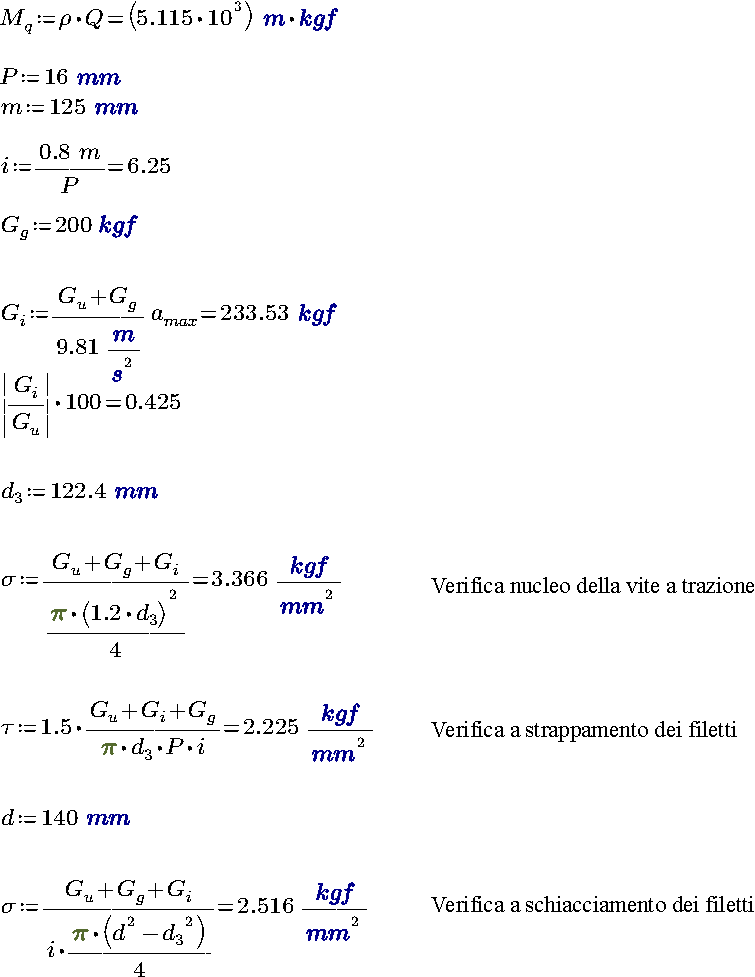
\includegraphics[width=.6\textwidth]{imgs/Mathcad7}
\caption{}
\label{fig:Mathcad7}
\end{figure}

\subsection{Verifica dei lamoni e dei piastroni}
\begin{figure}[H]
\centering
  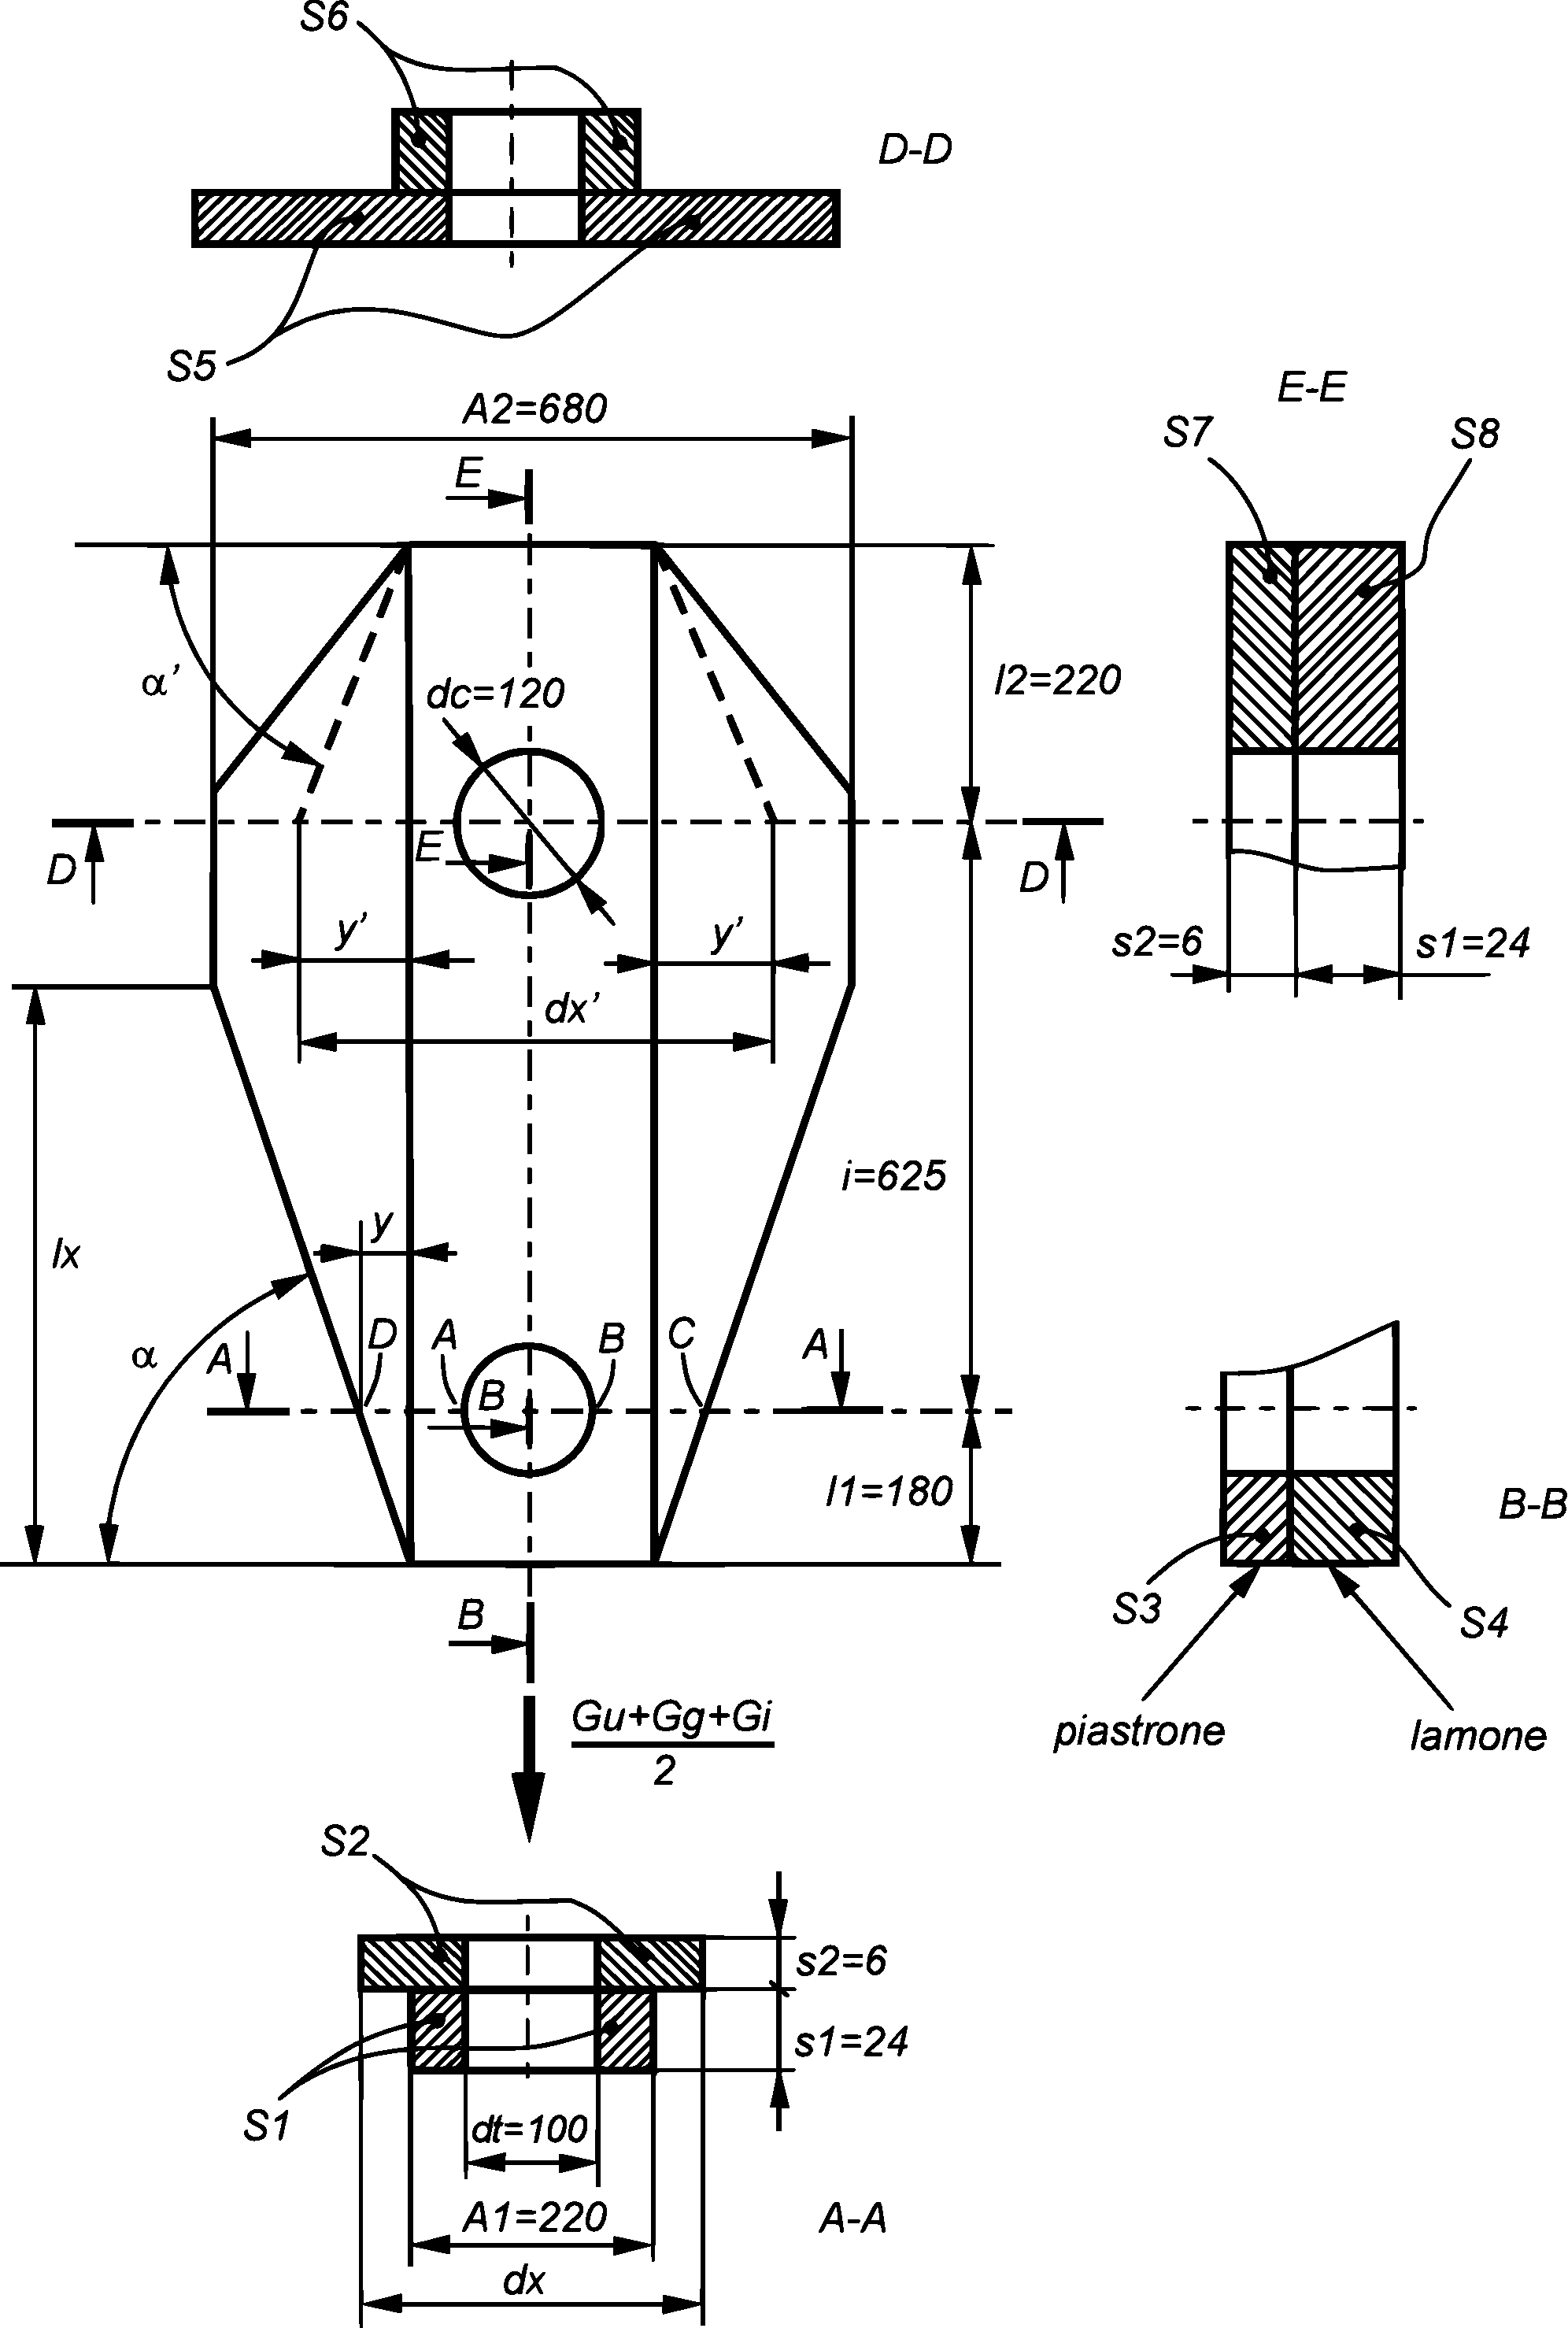
\includegraphics[width=.6\textwidth]{imgs/Cap6/3 LamPias}
\caption{Vista lamone-piastrone. Le quote non sono quelle utilizzate nei calcoli.}
\label{fig:LamPias}
\end{figure}
Prevedendo di usare tre carrucole e tenendo conto di un gioco assiale complessivo di $5\; mm$, l'ingombro assiale totale sarà di $3T+5 = 257 \; mm$ con $T$ ingombro assiale della singola carrucola fissato a $84 \;mm$. 
Per svolgere i seguenti calcoli si è utilizzato il modello di trave semplice appoggiata in cui le reazioni vengono modellate come forze distribuite lungo la generatrice del perno della traversa. 
Bisogna quindi conoscere anche la lunghezza dei perni che dipende dallo spessore di lamone e piastrone.
Si comincia dalla sezione A-A dei lamoni piastroni aventi spessori rispettivamente $s_1$ e $s_2$.
Viene considerata una ripartizione dello sforzo omogenea tra lamone e piastrone ma non viene effettuata una valutazione della sollecitazione su tutta l'area $S_1+S_2$ in quanto è noto che $S_2$ è molto inferiore a $S_1$.
Dopo aver calcolato l'area $S_1$ del piastrone è molto semplice valutare le $\sigma$ medie di trazione.
\begin{figure}[H]
\centering
  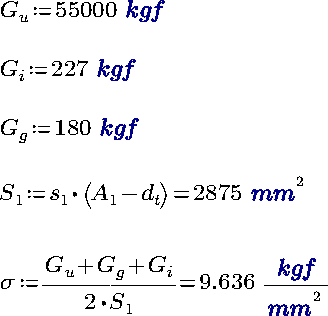
\includegraphics[width=.25\textwidth]{imgs/MathLP1}
\caption{}
\label{fig:MathLP1}
\end{figure}
\begin{figure}[H]
\centering
  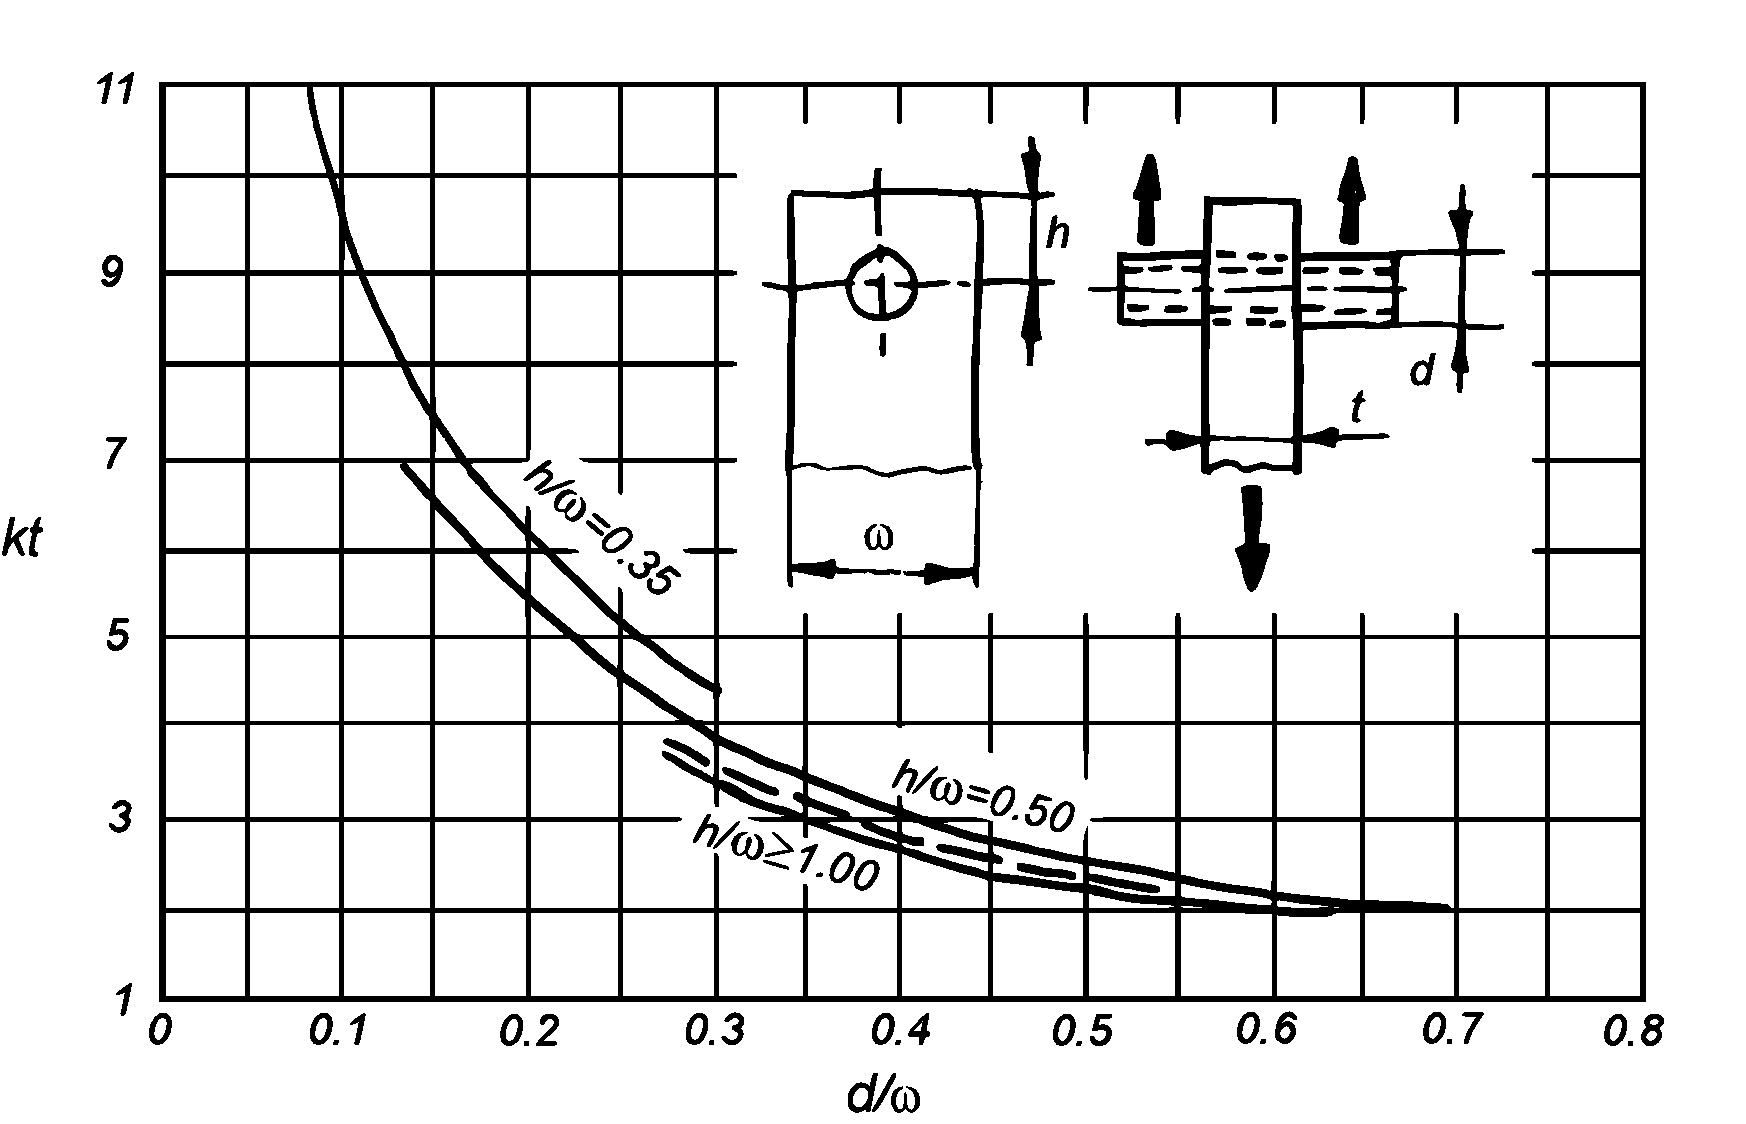
\includegraphics[width=.6\textwidth]{imgs/Cap6/4 FattoreForma}
\caption{Fattore di intaglio.}
\label{fig:FattoreForma}
\end{figure}
La presenza dei fori genera però un effetto intaglio. 
Determinare in maniera precisa l'entità della sovrasollecitazione rispetto al caso ideale non è semplice, in questa sede si fa riferimento alla figura \ref{fig:FattoreForma}. 
Come si vede, è riportato il coefficiente di sovrasollecitazione in funzione dei rapporti $d_t/A_1$ e $l_1/A_1$. 
La condizione di carico in figura non rispetta esattamente quella in analisi in quanto il carico risulta applicato solamente ad un lato del perno. 
Questa condizione di carico può quindi generare un aumento della sollecitazione nel bordo inferiore interno del foro del piastrone; per far si che il caso in figura sia più fedele a quello in esame, si dimensiona la traversa rendendola tozza in modo da limitare la flessione dei perni sotto carico. 
Un ulteriore discostamento dal caso ideale si ha per il fatto che il piastrone ha la parte terminale trapezia.
Questo fatto porta ad una sottostima dello sforzo nella zona sotto la linea che uniscie i punti $A$ e $B$ che non avrà più larghezza $dx$. 
A tal proposito si approssima l'angolo $\alpha$ a $70^\circ$, in questo modo si limita l'errore commesso. 
\begin{figure}[H]
\centering
  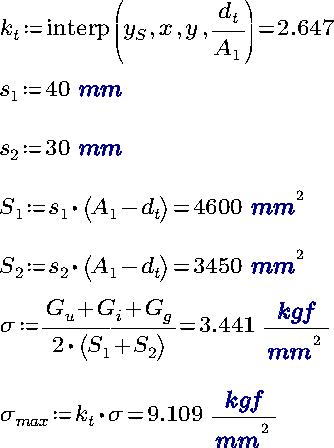
\includegraphics[width=.3\textwidth]{imgs/MathLP2}
\caption{}
\label{fig:MathLP2}
\end{figure}
Il valore ricavato inizialmente era sicuramente troppo elevato, nonostante il calcolo sia stato eseguito in favore di sicurezza trascurando il lamone. 
Un valore di solleciatazione ragionevole è compreso tra $9$ e $9.5 \; kgf/mm^2$. Per ovviare questo problema è stata aumentata la sezione di lamone e piastrone a rispettivamente $s_1=40 \; mm$ e $s_2=30 \; mm$. 
Si tratta di un valore ancora elevato ma è stato ricavato con calcoli in favore di sicurezza; si rimana al calcolo agli elementi finiti un'eventuale modifica delle quote. 

Viene fatta ora una nuova ipotesi: il carico si suppone ripartito ugualmente su lamone e piastrone. 
Questi due elementi sono rigidamente vincolati tra loro, la deformazione del foro comune sarà quindi principalmente longitudinale e identica per i due corpi.
Si può quindi calcolare il valore $dx$ minimo, compreso entro due limiti, affinchè la sollecitazione massima sia uguale sulle due aree $S_1$ e $S_2$.
\begin{figure}[H]
\centering
  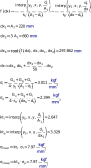
\includegraphics[width=.45\textwidth]{imgs/MathLP4}
\caption{}
\label{fig:MathLP4}
\end{figure}
Con il valore $dxs$ si calcolano le $\sigma_{max}$ sia sul lamone che sul piastrone per verificare che coincidano.
I valori ricavati sono sicuramente più accettabili dello sforzo massimo calcolato precedentemente. 

A questo punto si può calcolare l'angolo $\alpha$.
Il valore trovato è sicuramente accettabile.
\begin{figure}[H]
\centering
  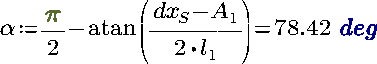
\includegraphics[width=.3\textwidth]{imgs/MathLP5}
\caption{}
\label{fig:MathLP5}
\end{figure}
\clearpage

\subsection{Dimensionamento e verifica della traversa}
Per il dimensionamento della taversa si fa riferimento alla tabella in figura \ref{fig:TabTraversa}.
Bisogna tenere conto del fatto che il gambo del gancio è stato dimensionato con $d=140$, la quota $d_2$ dovrà quindi essere modificata per permettere l'accoppiamento con gioco. Nella fase di analisi FEM queste quote sono state ulteriormente modificate per ovviare a problemi di concentrazione degli sforzi dovuti ai raccordi sui perni della traversa. 
Sono stati infatti aumentati i diametri dei perni e i raggi di raccordo degli stessi.
La pista è stata prevista avente diametro $1.1 \times d_{sfera}$.
La distanza tra bordo superiore ella traverssa e bordo inferiore del dado è di $11 \; mm$.
\begin{figure}[H]
\centering
\begin{minipage}{.5\textwidth}
  \centering
  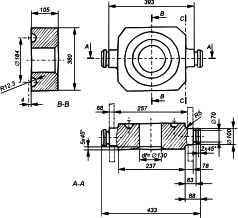
\includegraphics[width=.8\linewidth]{imgs/Cap6/5 SchizzoTraversa}
  \captionof{figure}{}
  \label{fig:SchizzoTraversa}
\end{minipage}%
\begin{minipage}{.5\textwidth}
  \centering
  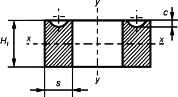
\includegraphics[width=.7\linewidth]{imgs/Cap6/7 SezResTrav}
  \captionof{figure}{}
  \label{fig:SezResTrav}
\end{minipage}
\end{figure}
\begin{figure}[H]
\centering
  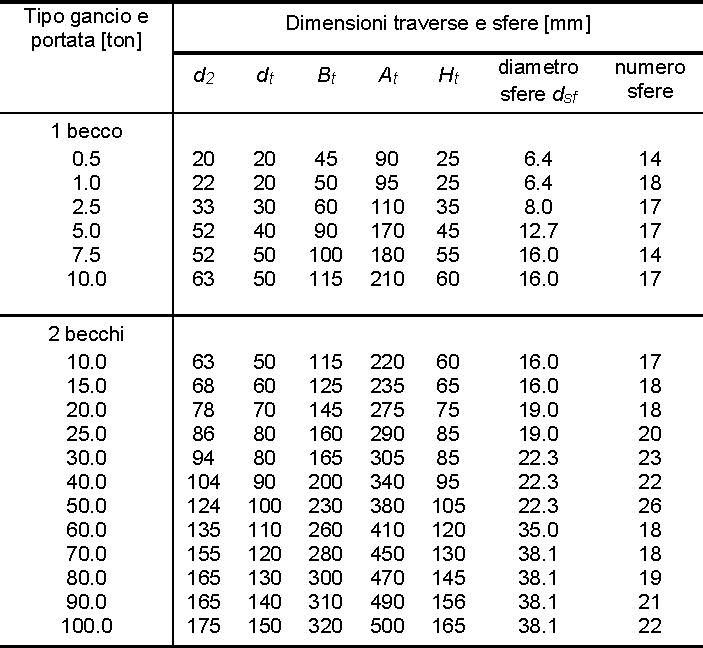
\includegraphics[width=.45\textwidth]{imgs/TabTraversa}
\caption{}
\label{fig:TabTraversa}
\end{figure}

\begin{table}[H]
\centering
\begin{tabular}{cccccccc}
\toprule
\begin{tabular}[c]{@{}c@{}}$d_2$\\ $[mm]$\end{tabular} & \begin{tabular}[c]{@{}c@{}}$d_t$ \\ $[mm]$\end{tabular} & \begin{tabular}[c]{@{}c@{}}$B_t$\\ $[mm]$\end{tabular} & \begin{tabular}[c]{@{}c@{}}$A_t$\\ $[mm]$\end{tabular} & \begin{tabular}[c]{@{}c@{}}$H_t$\\ $[mm]$\end{tabular} & \begin{tabular}[c]{@{}c@{}}$d_{sf}$\\ $[mm]$\end{tabular} & \begin{tabular}[c]{@{}c@{}}$n_s$\\ $[mm]$\end{tabular} & \begin{tabular}[c]{@{}c@{}}$d_{pista}$\\ $[mm]$\end{tabular} \\
\midrule
$130$                                                  & $105$                                                   & $245$                                                  & $395$                                                  & $113$                                                  & $29$                                                      & $22$                                                   & $188$                        \\
\bottomrule                               
\end{tabular}
\caption{Interpolazione dei valori nella tabella in figura\ref{fig:TabTraversa}. Nota: $d_{pista} = (d_2 + B_t)/2$}
\label{tab:InterpTraversa}
\end{table}

Si passa ora alle verifiche strutturali sulla traversa. Si fa riferimento al modello di carico ed i relativi diagrammi di sollecitazione mostrati in figura \ref{fig:DiagCarico}. 
\begin{figure}[H]
\centering
  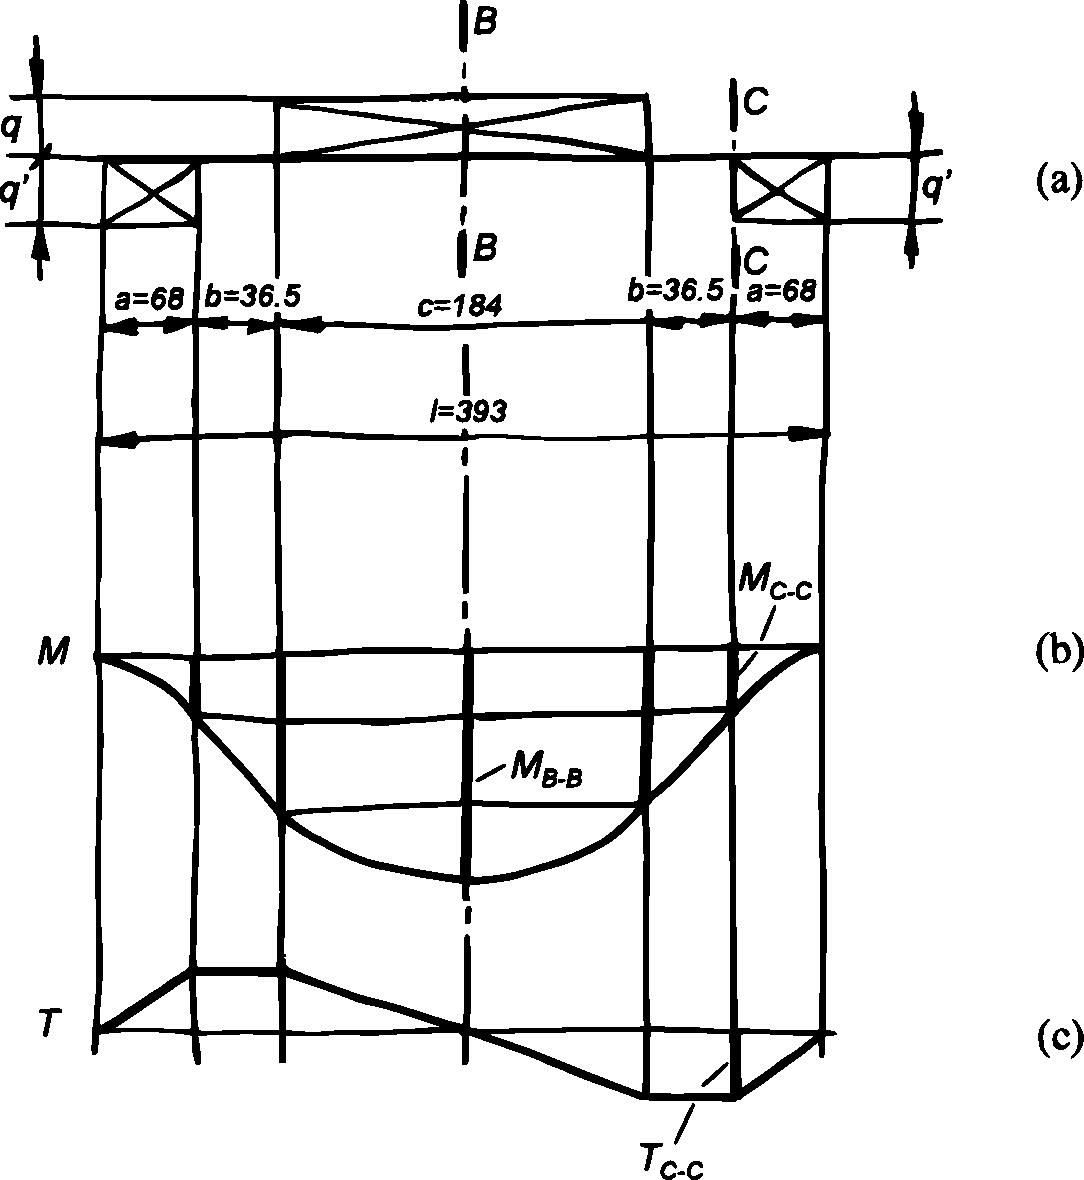
\includegraphics[width=.5\textwidth]{imgs/Cap6/6 DiagCarico}
\caption{}
\label{fig:DiagCarico}
\end{figure}
Si procede ora con la valutazione dello sforzo dovuto alla flessione in corrispondenza della sezione BB e la sollecitazione ideale massima nella sezione CC dovuta sia a flessione sia taglio.
\begin{figure}[H]
\centering
  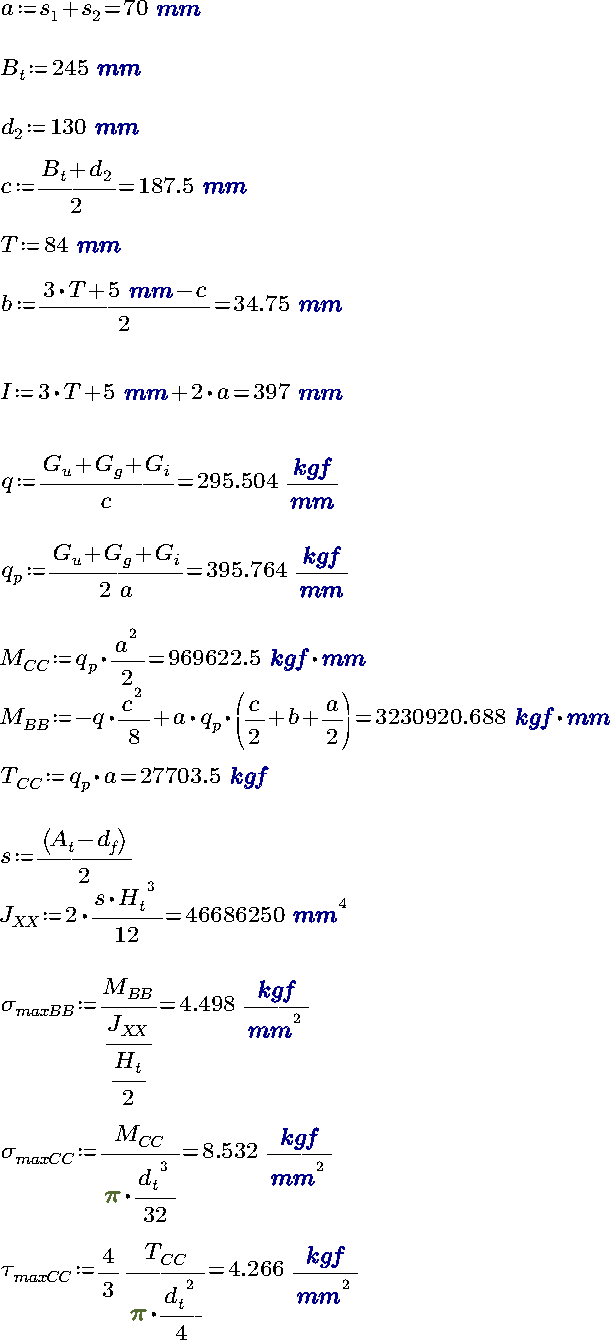
\includegraphics[width=.5\textwidth]{imgs/MathTrav1}
\caption{Calcolo momento flettente e $\sigma$ massime per sezioni BB e CC. Calcolo del taglio e $\tau$ massima nella sezione CC.}
\label{fig:MathTrav2}
\end{figure}
\begin{figure}[H]
\centering
  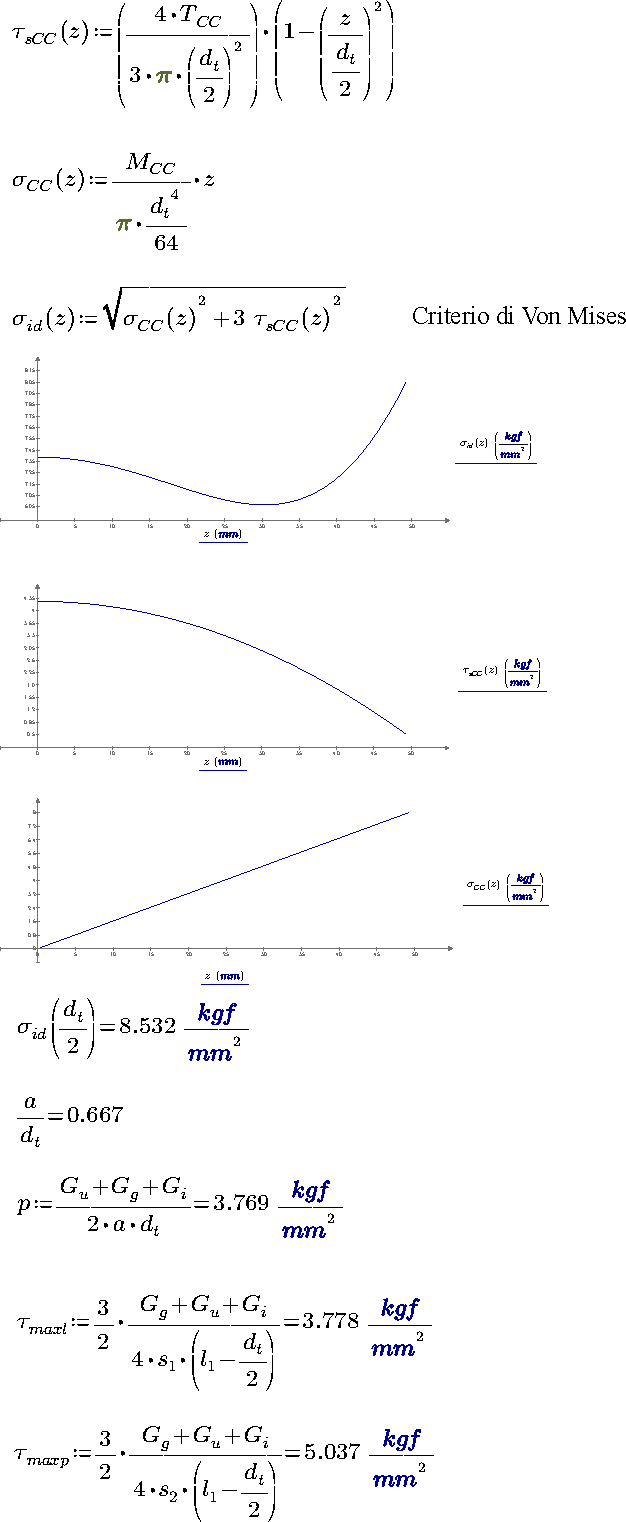
\includegraphics[width=.5\textwidth]{imgs/MathTrav2}
\caption{Calcolo della sollecitazione ideale massima e della pressione media di contatto relativamente al perno della traversa. Verifica a taglio sulla sezione BB.}
\label{fig:MathTrav2}
\end{figure}
Il rapporto $a/d_t$ è tale che i perni della traversa possano essere considerati tozzi.
Il comportamento anomalo di $\sigma_{id}$ è dato dalla presenza degli sforzi di taglio, i valori di questi ultimi sono però sotto i limiti imposti. 
Si è effettuata una valutazione della pressione media di contatto $p$ tra le superfici dei perni e dei fori. 
Per valutare l'ammissibilità di tale pressione si fa riferimento alla TABELLA, riferita ai valori di pressione ammessi relativamente a perni inseriti in cuscinetti a strisciamento.
Il valore delle pressioni medie è ammissibile. 

L'ultima verifica è stata effettuata al taglio nella sezione B-B supponendo il carico equidistribuito tra le sezioni $S_3$ e $S_4$ di lamone e piastrone. Si sono calcolate allora $\tau_{maxl}$ e $\tau_{maxp}$ che risultano accettabili.
La stessa procedura di calcolo per valutare la sezione A-A è stata ripetuta per valutare la sezione D-D. Anche in questo caso l'esito delle verifiche è positivo. 
In ultimo si procede con la verifica a taglio della sezione E-E come è stato fatto per la sezione B-B. 
\begin{figure}[H]
\centering
  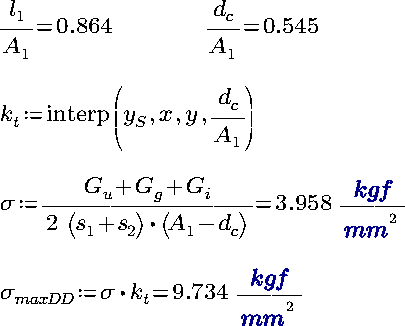
\includegraphics[width=.4\textwidth]{imgs/MathTrav3}
\caption{Calcolo della sollecitazione nella sezione D-D.}
\label{fig:MathTrav3}
\end{figure}

\begin{figure}[H]
\centering
  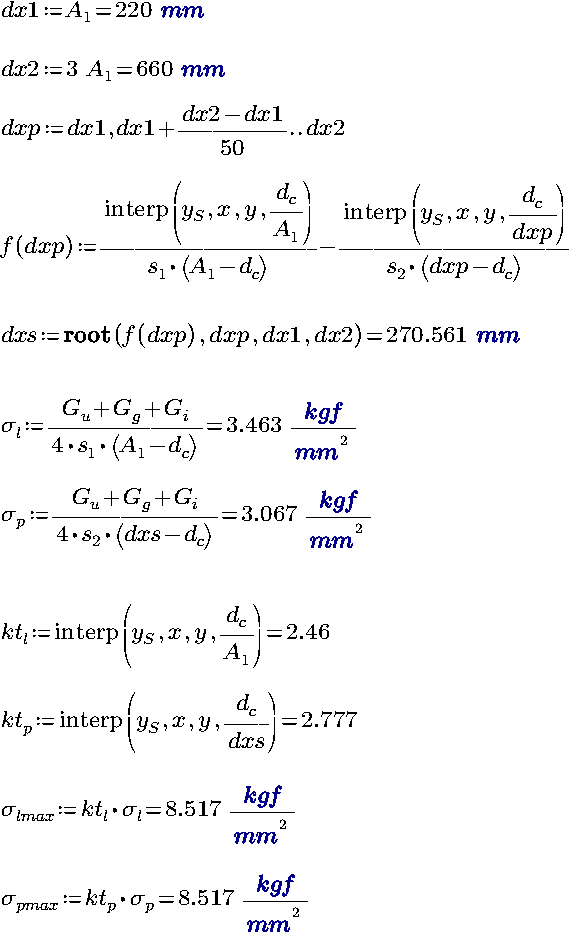
\includegraphics[width=.5\textwidth]{imgs/MathTrav4}
\caption{Sollecitazioni massime in D-D.}
\label{fig:MathTrav4}
\end{figure}

\begin{figure}[H]
\centering
  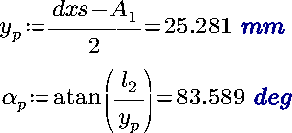
\includegraphics[width=.3\textwidth]{imgs/MathTrav5}
\caption{Calcolo di $\alpha'$.}
\label{fig:MathTrav5}
\end{figure}

\begin{figure}[H]
\centering
  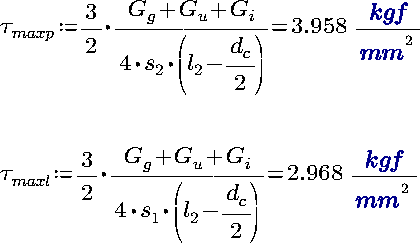
\includegraphics[width=.4\textwidth]{imgs/MathTrav6}
\caption{Verifica a taglio della sezione E-E.}
\label{fig:MathTrav6}
\end{figure}
\vfill
\clearpage
\subsection{Dimensionamento e verifica dell'asse delle carrucole}
L'ultimo elemento da dimensionare è l'asse porta carrucole. Il calcolo delle sollecitazioni tiene conto di flessione e taglio anche se quest'ultimo, si vedrà alla fine, non contribuirà a definire la massima sollecitazione dell'asse.
Si vanno a considerare tre sezioni resistenti come mostrato in figura \ref{fig:AsseDisegno}. 
Si vede che in quest'asse sono praticati dei fori ciechi che rappresentano i condotti di adduzione del grasso per la lubrificazione delle bussole calettate con interferenza nelle carrucole.
\begin{figure}[H]
\centering
  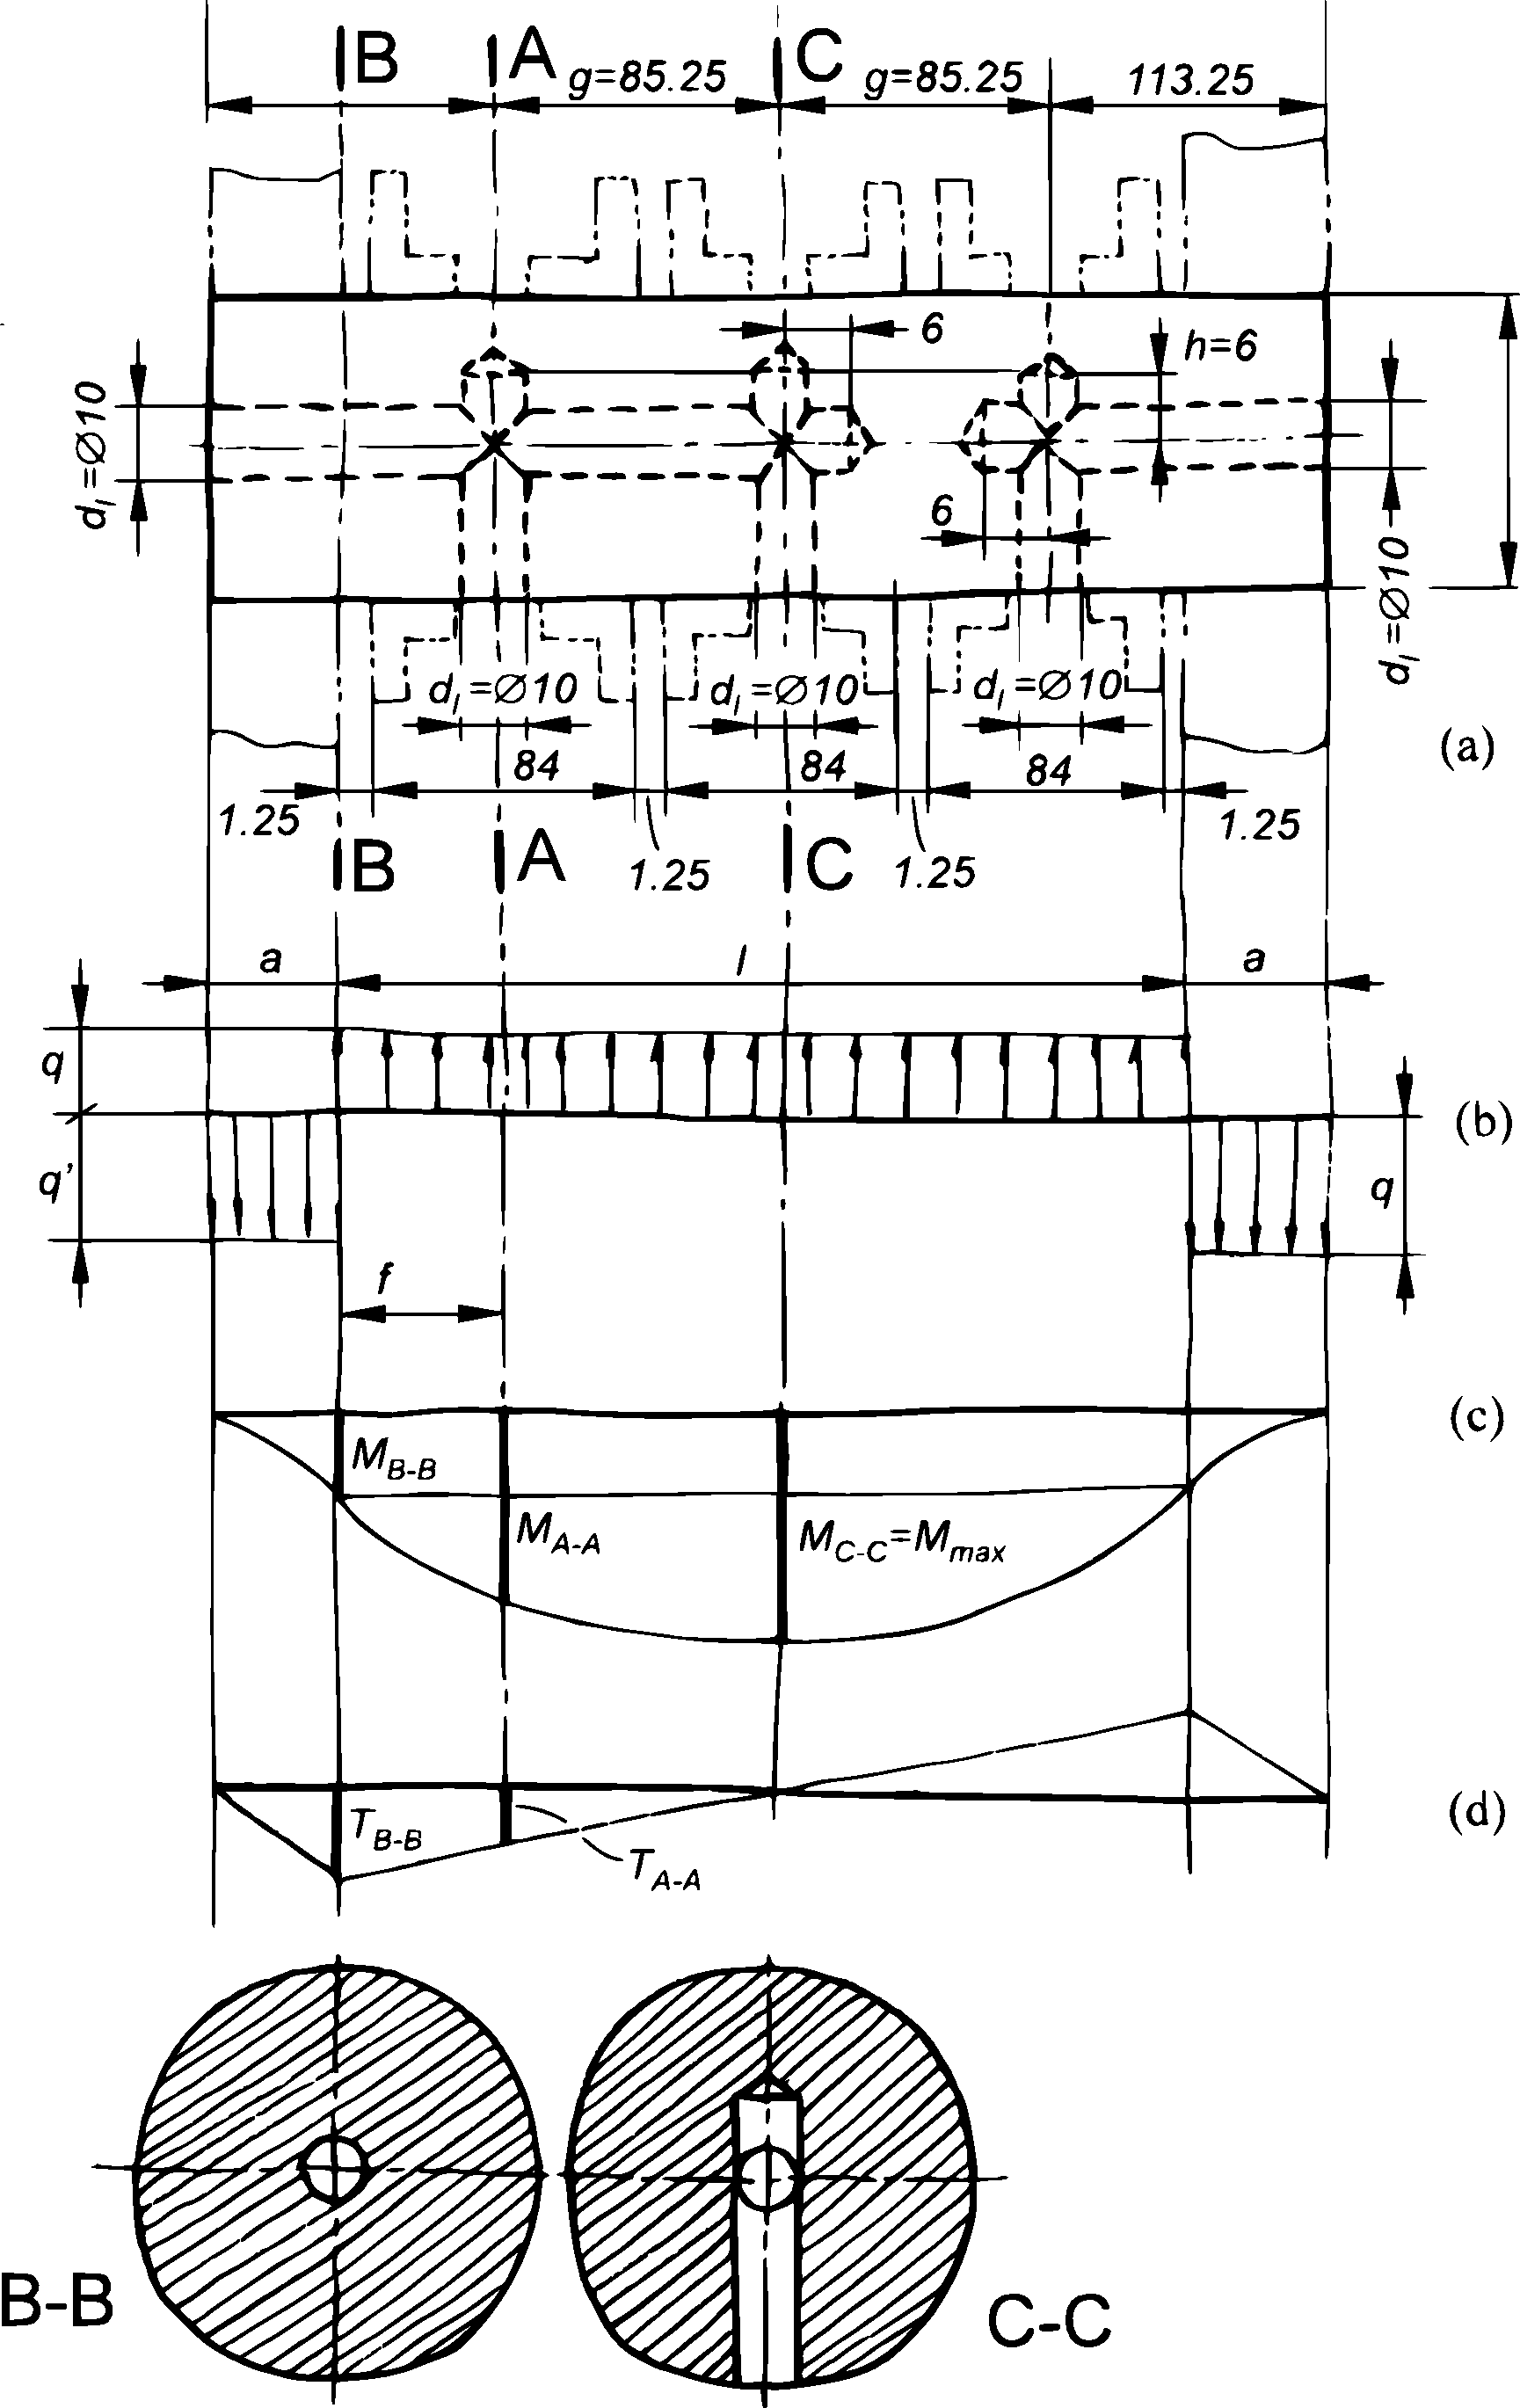
\includegraphics[width=.7\textwidth]{imgs/AsseDisegno}
\caption{}
\label{fig:AsseDisegno}
\end{figure}
Si ipotizza che le suddette bussole applichino un carico uniformemente distribuito $q$ sull'intera lunghezza $l$ della superficie compresa entro i lamoni-piastroni. 
In realtà le bussole si estendono per tre tratti distinti come illustrato in figura \ref{fig:AsseDisegno}, si ricorda inoltre che è stato previsto un gioco assiale di $5$ $mm$ per permettere il corretto funzionamento del bozzello. 
Il modello proposto è sicuramente in favore di sicurezza in quanto sovrastima il carico agente sull'asse e semplifica notevolmente il calcolo dei momenti flettenti. 
Si può allora definire un carico $q$ agente su tutta la lunghezza $l$
\begin{align*}
q = \frac{G_u+G_i+G_g}{l'}
\end{align*}
Con $l'$ lunghezza effettiva di contatto asse-boccole. 
A questo punto con $q'$ si indica il carico distribuito applicato sulle superfici dei fori dei lamoni-piastroni. Per garantire l'equilibrio 
\begin{align*}
2 \: q' \; a = q \; l
\end{align*}
Basandosi sui diagrammi di carico in figura, si è deciso di verificare le sezioni A-A, B-B e C-C. Nella sezione A-A si è calcolata una $\sigma$ ideale massima con il criterio di Huber, combinando l'effetto del momento flettente $M_{AA}$ e del taglio $T_{AA}$. Questa sezione resistente è indebolita dal foro radiale di adduzione del grasso e per giunta si trova notevolmente sollecitata. Per gli stessi motivi si controlla la sezione B-B, il momento flettente è minore rispetto al caso precedente ma lo sforzo di taglio è non nullo. 
Nella sezione C-C il taglio è nullo ma si ha massimo momento flettente $M_{C-C}$  e la sezione è ancora indebolita dal foro di lubrificazione. 

Per il calcolo delle $\sigma$ di flessione e delle corrispondenti $\tau$ occorre, per ogni sezione, definire la posizione dei baricentri e il valore delle aree delle sezioni stesse, l'asse neutro, i momenti statici e i momenti quadratici di superficie (sempre rispetto all'asse neutro). 
Bisogna inoltre, per calcolare le $\tau$ in maniera puntuale, definire un momento statico dell'area sottesa inferiormente ad una corda che taglia la sezione in esame. 
Per semplicità di calcolo si considera questa corda sempre parallela all'asse neutro, in corrispondenza di essa si va a calcolare il valore di $\tau$. 
Traslando verticalmente questa corda (definita parametricamente secondo una coordinata verticale) si ottengono le $\tau$ massime correnti, avendo $\sigma$ di flessione si può calcolare la $\sigma$ ideale con il criterio di Huber. 

\begin{figure}[H]
\centering
  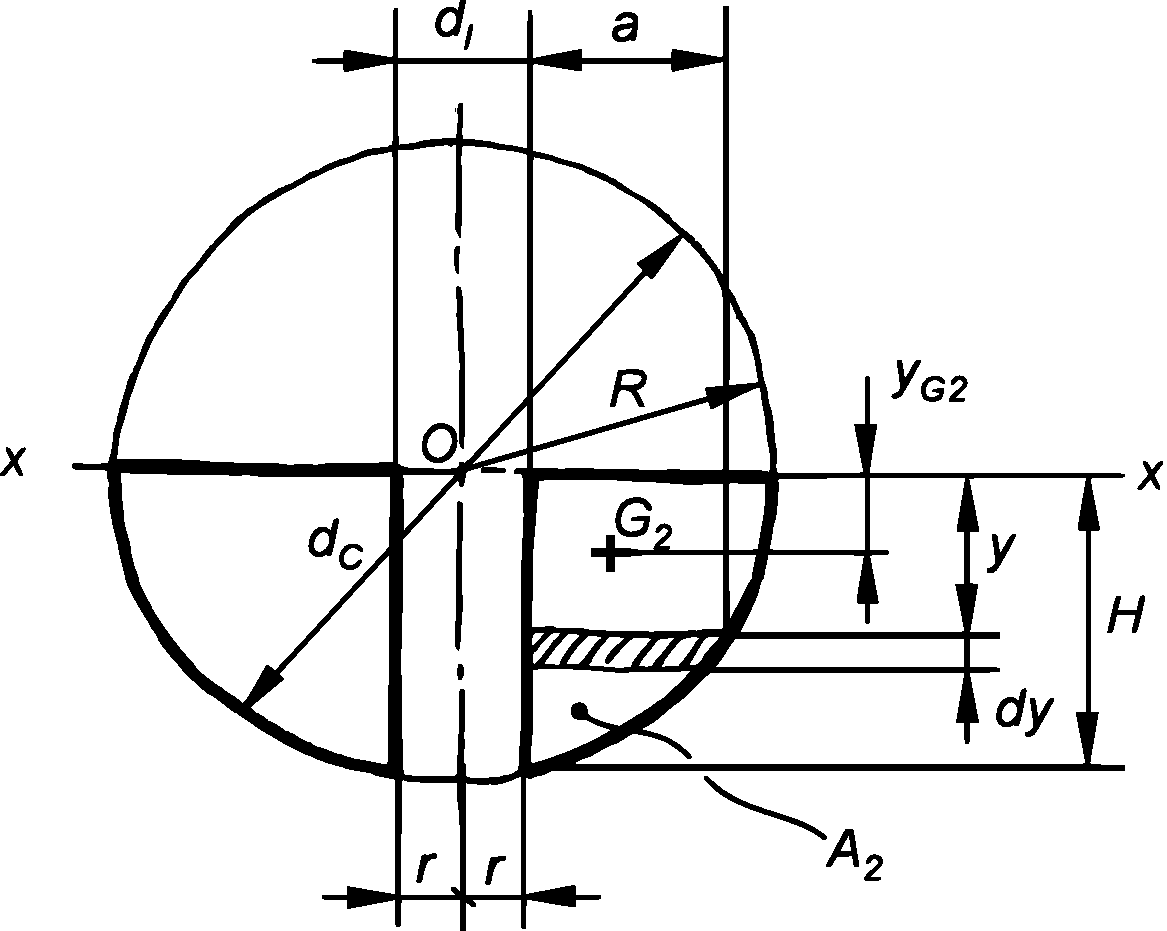
\includegraphics[width=.35\textwidth]{imgs/Cap7/SezAsse1}
\caption{Parte inferiore della sezione A-A.}
\label{fig:SezAsse1}
\end{figure}
Si procede con il calcolo del momento statico riferito alle sezioni A-A e C-C dell'area $A_2$ in figura \ref{fig:SezAsse1}.
Si possono poi calcolare l'area $A_2$ e il baricentro $y_{G2}$.
\begin{figure}[H]
\centering
  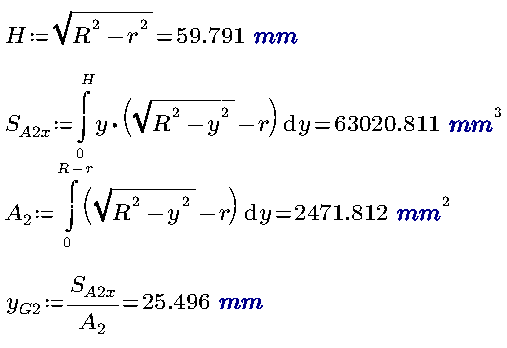
\includegraphics[width=.4\textwidth]{imgs/MathAsse1}
\caption{}
\label{fig:MathAsse1}
\end{figure}
\begin{figure}[H]
\centering
  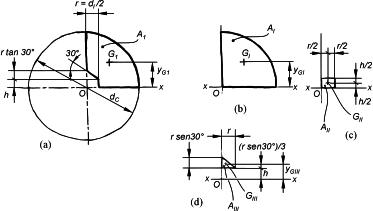
\includegraphics[width=.55\textwidth]{imgs/Cap7/SezAsse2}
\caption{Parte superiore delle sezioni A-A e C-C.}
\label{fig:SezAsse2}
\end{figure}
Si calcolano ora le aree $AI$, $AII$, $AIII$ e $A1$ in figura \ref{fig:SezAsse2} ed i relativi baricentri.
\begin{figure}[H]
\centering
  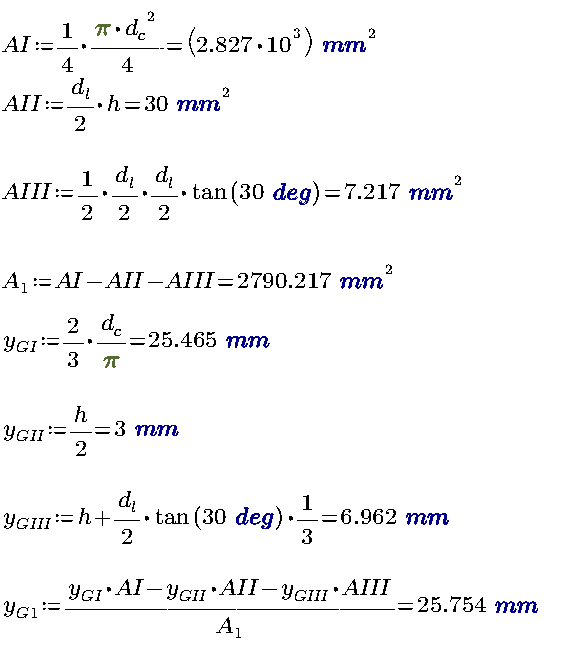
\includegraphics[width=.4\textwidth]{imgs/MathAsse2}
\caption{}
\label{fig:MathAsse2}
\end{figure}
\begin{figure}[H]
\centering
  \includegraphics[width=.35\textwidth]{imgs/Cap7/SezAsse3}
\caption{Sezioni A-A e C-C, determinazione del baricentro.}
\label{fig:SezAsse3}
\end{figure}
A questo punto è possibile calcolare l'ordinata $y_G$ del baricentro $G$ della sezione completa in figura \ref{fig:SezAsse3}.
\begin{figure}[H]
\centering
  \includegraphics[width=.3\textwidth]{imgs/MathAsse2_1}
\caption{}
\label{fig:MathAsse2_1}
\end{figure}
\begin{figure}[H]
\centering
  \includegraphics[width=.55\textwidth]{imgs/Cap7/SezAsse4}
\caption{Calcolo del momento quadratico di superficie (a) dell’area $A_2$ e (b) dell’area $A’_1$ rispetto all’asse neutro n-n relativamente alle sezioni A-A e C-C.}
\label{fig:SezAsse4}
\end{figure}
\begin{figure}[H]
\centering
  \includegraphics[width=.4\textwidth]{imgs/Cap7/SezAsse5}
\caption{Calcolo dei momenti quadratici di superficie dell’area $J_{tn}$ e $J_{rn}$.}
\label{fig:SezAsse5}
\end{figure}
A questo punto si calcola il momento di inerzia $J_{ACn}$ valutato rispetto all'asse neutro n-n della sezione in figura \ref{fig:SezAsse4}. Si fraziona l'area i figure più semplici, si calcolano i diversi momenti di inerzia a si sommano algebricamente. 
\begin{figure}[H]
\centering
  \includegraphics[width=.7\textwidth]{imgs/MathAsse3}
\caption{}
\label{fig:MathAsse3}
\end{figure}
Si calcolano quindi il momento d'inerzia $J_{XX}$ della sezione circolare completa calcolato rispetto all'asse diametrale e la riduzione percentuale $p$ del momento di inerzia della sezione dovuta alla presenza dei fori di adduzione del grasso.
\begin{figure}[H]
\centering
  \includegraphics[width=.3\textwidth]{imgs/MathAsse3_1}
\caption{}
\label{fig:MathAsse3_1}
\end{figure}
Adesso viene definito il momento statico rispetto all'asse neutro n-n dell'area sottesa da una generica corda di lunghezza $b_r$ avente ordinata $y_{br}$ che attraversa orizzontalmente la sezione in esame. 
Per semplicità di calcolo si analizzano tre casi:
\begin{enumerate}
\item $-(h-y_G) \leq y_{br} \leq H+y_G$
\item $-(r \cdot \tan(30^\circ)+h-y_G) \leq y_{br} \leq -(h-y_G)$
\item $-(R-y_G) \leq y_{br} \leq -r \cdot \tan(30^\circ)-(h-y_G)$
\end{enumerate}

\subsubsection{$-(h-y_G) \leq y_{br} \leq H+y_G$}
\begin{figure}[H]
\centering
  \includegraphics[width=.4\textwidth]{imgs/Cap7/SezAsse6}
\caption{Calcolo del momento statico dell'area sottesa dalla corda $b_r$ al di sotto della base dello scavo conico relativamente alle sezioni A-A e C-C.}
\label{fig:SezAsse6}
\end{figure}
Si indica con $S_{1An}$ il momento statico sotteso dalla corda $b_r$. 
\begin{figure}[H]
\centering
  \includegraphics[width=.4\textwidth]{imgs/MathAsse4_0}
\caption{}
\label{fig:MathAsse4_0}
\end{figure}
Si calcolano le $\tau$ massime di taglio sulla corda $b_r$ in figura \ref{fig:SezAsse7}.
Innanzitutto si valuta la componente verticale costante $\tau_{zym}$ che rappresenta il valore medio delle tensioni di taglio, ragionevolmente poco diversa dalla tensione tangenziale per ogni punto di $b_r$. 
Per il calcolo degli sforzi di taglio bisogna prima calcolare il taglio $T_{AA}$. Nel farlo si fa riferimento al carico distribuito $q_s$ lungo la lunghezza $I$ e non il carico distribuito $q$ lungo $I'$. Come si vede nei calcoli, la sovrastima è del $17\%$. 
\begin{figure}[H]
\centering
  \includegraphics[width=.45\textwidth]{imgs/Cap7/SezAsse7}
\caption{Calcolo del momento statico dell’area sottesa dalla corda br posta tra l’asse neutro n-n e il vertice dello scavo conico relativamente alle sezioni A-A e C-C.}
\label{fig:SezAsse7}
\end{figure}
\begin{figure}[H]
\centering
  \includegraphics[width=.65\textwidth]{imgs/MathAsse4}
\caption{}
\label{fig:MathAsse4}
\end{figure}
Di seguito è riportato l'andamento di $\tau_{zym}$.
\begin{figure}[H]
\centering
  \includegraphics[width=.65\textwidth]{imgs/MathAsse4_1}
\caption{}
\label{fig:MathAsse4_1}
\end{figure}
A questo punto si può valutare la tensione tangenziale $\tau_z$ che si rileva essere massima nel contorno esterno, leggermente sopra l'asse neutro. 
\begin{figure}[H]
\centering
  \includegraphics[width=.65\textwidth]{imgs/MathAsse4_2}
\caption{}
\label{fig:MathAsse4_2}
\end{figure}

\begin{figure}[H]
\centering
  \includegraphics[width=.45\textwidth]{imgs/Cap7/SezAsse8}
\caption{Calcolo del momento statico dell’area sottesa dalla corda br posta tra l’asse neutro n-n e il vertice dello scavo conico relativamente alle sezioni A-A e C-C.}
\label{fig:SezAsse8}
\end{figure}

\subsubsection{$-(r \cdot \tan(30^\circ)+h-y_G) \leq y_{br} \leq -(h-y_G)$}
\begin{figure}[H]
\centering
  \includegraphics[width=.45\textwidth]{imgs/Cap7/SezAsse9}
\caption{Calcolo del momento statico dell’area sottesa dalla corda br posta tra l’asse neutro n-n e il vertice dello scavo conico relativamente alle sezioni A-A e C-C.}
\label{fig:SezAsse9}
\end{figure}
\begin{figure}[H]
\centering
  \includegraphics[width=.75\textwidth]{imgs/MathAsse5_0}
\caption{}
\label{fig:MathAsse5_0}
\end{figure}
Si calcolano $\tau'_z$ e $\tau''_z$, sollecitazioni rispettivamente sul contorno interno ed esterno.
\begin{figure}[H]
\centering
  \includegraphics[width=.4\textwidth]{imgs/Cap7/SezAsse10}
\caption{Calcolo del momento statico dell’area sottesa dalla corda br posta tra l’asse neutro n-n e il vertice dello scavo conico relativamente alle sezioni A-A e C-C.}
\label{fig:SezAsse10}
\end{figure}
Per quanto riguarda il calcolo di $\tau'$, bisogna considerare $\alpha=30^\circ$ mentre per $\tau''$ sarà pari a 
\begin{align*}
\alpha(y_{br}) = \arctan \left( \frac{|y_{br}|+y_G}{b_r(y_{br})+\frac{|y_{br}|-(h-y_G}{\tan(30)}} \right)
\end{align*}
\begin{figure}[H]
\centering
  \includegraphics[width=.45\textwidth]{imgs/Cap7/SezAsse11}
\caption{Calcolo del momento statico dell’area sottesa dalla corda br posta tra l’asse neutro n-n e il vertice dello scavo conico relativamente alle sezioni A-A e C-C.}
\label{fig:SezAsse11}
\end{figure}
\begin{figure}[H]
\centering
  \includegraphics[width=.75\textwidth]{imgs/MathAsse5_2}
\caption{}
\label{fig:MathAsse5_2}
\end{figure}
Il valore massimo di sollecitazione si rileva sul contorno interno in corrispondenza a $y_{br} = -(h-y_G)$. 

\subsubsection{$-(R-y_G) \leq y_{br} \leq -r \cdot \tan(30^\circ)-(h-y_G)$}
\begin{figure}[H]
\centering
  \includegraphics[width=.4\textwidth]{imgs/Cap7/SezAsse12}
\caption{Calcolo del momento statico dell’area sottesa dalla corda br posta tra l’asse neutro n-n e il vertice dello scavo conico relativamente alle sezioni A-A e C-C.}
\label{fig:SezAsse12}
\end{figure}
\begin{figure}[H]
\centering
  \includegraphics[width=.6\textwidth]{imgs/MathAsse6_0}
\caption{}
\label{fig:MathAsse6_0}
\end{figure}
Si calcolano gli sforzi di taglio $\tau_z$ come nei casi precedenti. 
\begin{figure}[H]
\centering
  \includegraphics[width=.25\textwidth]{imgs/MathAsse6_1}
\caption{}
\label{fig:MathAsse6_1}
\end{figure}
\begin{figure}[H]
\centering
  \includegraphics[width=.75\textwidth]{imgs/MathAsse6_2}
\caption{}
\label{fig:MathAsse6_2}
\end{figure}
Il massimo valore di sollecitazione si ha in corrispondenza dello scavo conico. Il comportamento di $\tau_z$ che assume in corrispondenza di $-(R-y_G)$ è dovuto ad una singolarità numerica: $\alpha$ tende a $90^\circ$, il denominatore tende quindi a $0$. 

\subsubsection{Verifica della sezione B-B}
Si passa ora allo studio della sezione B-B (figura \ref{fig:SezAsse13}). Si vanno a calcolare nell'ordine:
\begin{itemize}
\item Il momento statico dell'area sottesa dalla corda $b_{r1}$ quando la stessa si trova tra asse neutro n-n e la tangente all'orizzontale alla circonferenza di raggio r;
\item il momento statico dell'area sottesa dalla corda $b_{r2}$ quando la stessa si trova tra le due tangenti orizzontali alle circonferenze di raggi $r$ e $R$.
\end{itemize}
Si può quindi calcolare il taglio $T_{BB}$ e il momento di inerzia della sezione B-B $J_{Bn}$. In questo modo si calcola la $\tau_{zym}$ e se ne grafica l'andamento nell'intervallo $0 \leq y_{br} \leq r$.
\begin{figure}[H]
\centering
  \includegraphics[width=.7\textwidth]{imgs/Cap7/SezAsse13}
\caption{}
\label{fig:SezAsse13}
\end{figure}
\begin{figure}[H]
\centering
  \includegraphics[width=.65\textwidth]{imgs/MathAsse7}
\caption{}
\label{fig:MathAsse7}
\end{figure}
Facendo riferimento alla figura \ref{fig:SezAsse14} si possono calcolare gli angoli $\alpha$ e $\alpha'$. A questo punto si possono calcolare le tensioni tangenziali sul contorno esterno e interno, rispettivamente $\tau_z$ e $\tau'_z$.
\begin{figure}[H]
\centering
  \includegraphics[width=.8\textwidth]{imgs/Cap7/SezAsse14}
\caption{}
\label{fig:SezAsse14}
\end{figure}
\begin{figure}[H]
\centering
  \includegraphics[width=.75\textwidth]{imgs/MathAsse7_1}
\caption{}
\label{fig:MathAsse7_1}
\end{figure}
Si vede che $\tau'_z$  diverge per $y_{Zbr}=r$ in quanto anche in questo caso il termine $\cos \alpha'$ tende a zero. Questo modello non è quindi applicabile, nell'intervallo considerato, nemmeno come approssimazione. 
Data la simmetria della sezione, la sollecitazione può essere studiata solo su metà di essa, in questo modo è possibile continuare ad utilizzare questo modello. 
Si nota come in figura \ref{fig:SezAsse15} (a) la componente $\tau_{zym}$ abbia andamento costante e non si possa dire lo stesso per la figura \ref{fig:SezAsse15} (b)
\begin{figure}[H]
\centering
  \includegraphics[width=0.9\textwidth]{imgs/Cap7/SezAsse15}
\caption{}
\label{fig:SezAsse15}
\end{figure}
\begin{figure}[H]
\centering
  \includegraphics[width=.68\textwidth]{imgs/MathAsse8_0}
\caption{}
\label{fig:MathAsse8_0}
\end{figure}
\begin{figure}[H]
\centering
  \includegraphics[width=.68\textwidth]{imgs/MathAsse8_1}
\caption{}
\label{fig:MathAsse8_1}
\end{figure}
Di seguito il calcolo delle sollecitazioni massime nelle varie sezioni, si fa riferimento alle tensioni presenti sul contorno esterno (tensioni massime), rispettivamente in $0 \leq y_{br} \leq r $ e $ r \leq y_{br} \leq R$.
\begin{figure}[H]
\centering
  \includegraphics[width=.68\textwidth]{imgs/MathAsse8_2}
\caption{}
\label{fig:MathAsse8_2}
\end{figure}

\subsubsection{Verifica nominale delle sollecitazioni ideali sull'asse delle carrucole}
Si valutano ora le $\sigma$ delle sezioni utilizzando il criterio di Huber. 

\textbf{Sezione B-B}\\[1mm]
Di seguito il grafico di $\sigma_{BB}$ al variare di $y_{br}$. Con le $\tau_{z1}$ e $\tau_{z2}$ si potranno calcolare le $\sigma_{BBid}$.
\begin{figure}[H]
\centering
  \includegraphics[width=.68\textwidth]{imgs/MathAsse9_0}
\caption{}
\label{fig:MathAsse9_0}
\end{figure}
\begin{figure}[H]
\centering
  \includegraphics[width=.68\textwidth]{imgs/MathAsse9_1}
\caption{}
\label{fig:MathAsse9_1}
\end{figure}
La verifica ha avuto esito positivo.

\textbf{Sezione A-A}\\[1mm]
$0 \leq y_{br} \leq H+y_G$
\begin{figure}[H]
\centering
  \includegraphics[width=.68\textwidth]{imgs/MathAsse9_2}
\caption{}
\label{fig:MathAsse9_2}
\end{figure}
$- \left(h-y_G \right) \leq y_{br} \leq 0$
\begin{figure}[H]
\centering
  \includegraphics[width=.68\textwidth]{imgs/MathAsse9_3}
\caption{}
\label{fig:MathAsse9_3}
\end{figure}
$- \left(h-y_G \right) \leq y_{br} \leq - \left( h - y_G + r \cdot \tan 30^{\circ} \right)$
\begin{figure}[H]
\centering
  \includegraphics[width=.7\textwidth]{imgs/MathAsse9_4}
\caption{}
\label{fig:MathAsse9_4}
\end{figure}
$- \left( R - y_G \right) \leq y_{br} \leq - \left( h - y_G + r \cdot \tan 30^{\circ} \right)$
\begin{figure}[H]
\centering
  \includegraphics[width=.7\textwidth]{imgs/MathAsse9_5}
\caption{}
\label{fig:MathAsse9_5}
\end{figure}


Nell'ultimo grafico si vede il valore di $\sigma_{4AAid}$ divergere a causa della differente velocità con cui tendono a $0$ i termini coinvolti.
In realtà si ha $\sigma_{4AAid}\left(-\left(R-y_G \right) \right) \equiv \sigma_{AA}\left(-\left(R-y_G \right) \right)$.

Il massimo valore di sollecitazione ($\sigma_{1AAid}\left(H+y_G \right)$) si ha nelle fibre più lontane dall'asse neutro nella zona in cui parte il foro cieco. 
Tale valore è di poco più alto del valore posto indicativamente come soglia.
In questa fase lo si considera comunque accettabile e si rimanda alla fase successiva un'eventuale modifica delle quote. 

\textbf{Sezione C-C}\\[1mm]
In questo caso il taglio è nullo ed il momento flettente è massimo. 
Il valore della sollecitazione ideale massima sarà $\sigma_{CCidmax} := \sigma_{CCmax} = 23.26 \;kgf/mm^2$.

\subsection{Verifica a fatica}
Si suppone l'utilizzo di un acciaio non legato con percentuale di carbonio allo $0.52\%$.
Le prove effettuate su provini\footnote{Il provino ha diametro $d=10\; mm$. G. Colombo, Nuovo Colombo, Manuale dell’Ingegnere,
vol. I, Ultima Edizione, Hoepli, Milano, pagg. C118-C119, Tabella 2} forniscono un limite a fatica pari a $\sigma_{FAf}= 38 \; kgf/mm^2$. 
A questo valore bisogna applicare dei coefficienti correttivi\footnote{Per $b$ si fa riferimento a C. Malavasi, Vademecum per l’Ingegnere Costruttore Meccanico, XV Edizione, Hoepli, Milano. Per $b_2$ si fa riferimento a E. Massa, Costruzione di Macchine, vol. I, Masson, Milano 1976, pag. 335.} per tenere conto dell'effetto scala e della finitura superficiale. 
Si sono scelti, attraverso un'interpolazione, i valori di $b=0.6$ e $b_2=0.9$.
Si ha quindi 
\begin{align*}
\sigma_{FAf} \cdot b \cdot b_2= 20.52 \; kgf/mm^2
\end{align*}
Bisogna però considerare che l'asse è soggetto a flessione pulsante dallo zero (con ragionevole approssimazione). 
Per determinare il limite a fatica $\sigma_{pFPf}$ alla flessione pulsante dallo zero si può tracciare il diagramma di Smith per l'acciaio considerato. 
Per procedere in questa direzione sono stati ricavati i dati presenti in tabella \ref{tab:smith}. Il dato di carico di rottura statico a flessione $\sigma_{Rf}$ non è presente nelle tabelle del manuale, si può assumere ragionevolmente pari al carico di rottura statica a trazione, si ha quindi $\sigma_{Rf} = 76.5 \; Kgf/mm^2$. 
\begin{table}[H]
\centering
\begin{tabular}{ll}
\toprule
$\sigma_{Rf}$                              & $76.5\;kg/mm^2$ \\
$\sigma_{snf}$                             & $45\;kg/mm^2$   \\
$\sigma_{FAf}$                             & $38\;kg/mm^2$   \\
$\sigma_{pFAf}$                            & $19.9\;kg/mm^2$ \\
$\sigma_{med}= \cfrac{\sigma_{CCidmax}}{2}$ & $10.6\;kg/mm^2$ \\
$k_1$                                      & $2$             \\
$\beta=\arctan (k_1)$                      & $63.4^{\circ}$  \\
$\gamma = \arctan \left(\frac{\sigma_{Rf} - \sigma_{pFAf}}{\sigma_{Rf}}\right)$                                   & $36.5^{\circ}$ \\
\bottomrule
\end{tabular}
\caption{Valori per il tracciamento del diagramma di Smith.}
\label{tab:smith}
\end{table}
Si può allora seguire il seguente procedimento, facendo riferimento alla figura \ref{tab:smith} si scrivono le seguenti relazioni
\begin{align*}
\frac{\sigma'_{FPf} - \sigma'_{FAf}}{\sigma_{med}+x} = \tan \gamma
\end{align*}
\begin{align*}
\frac{\sigma'_{FPf}}{\sigma_{med}+x} = \tan \beta
\end{align*}
Mettendo a sistema e risolvendo per $x$ e $\sigma_{pFPf}$ si ottiene
\begin{align*}
\sigma_{pFPf} = \frac{\sigma_{pFAf} \cdot \tan (\beta)}{\tan (\beta) - \tan (\gamma)} = 31.6 \; kgf/mm^2
\end{align*}
Il limite qui trovato supera il valore massimo di sollecitazione $\sigma_{CCidmax}$ del $35\%$. Il risultato ottenuto si può ragionevolmente considerare accettabile, la verifica a fatica è conclusa.
\begin{figure}[H]
\centering
  \includegraphics[width=.6\textwidth]{imgs/Smith}
\caption{Diagramma di Goodman-Smith.}
\label{fig:Smith}
\end{figure}
 